%%%%%%%%%%%%%%%%%%%%%%%%%%%%%%  IEEEsample.tex
%%%%%%%%%%%%%%%%%%%%%%%%%%%%%%%%%%%%%%%%%
%%%%%%%%%%%%%%%%%%%%%%%    More information: see the header of IEEEtran.sty
%%%%%%%%%%%%%%%%%%%%%%%
%%%%%%%%%%%%%%%%%%%%%%%%%%%%%%%%%%%%%%%%%%%%%%%%%%%%%%%%%%%%%%%%%%%%%%%%%%%%%%%%
%%%%

\documentclass[10pt,twocolumn]{IEEEtran}
%\documentclass[conference]{IEEEtran}

%%%\IEEEoverridecommandlockouts


%% set page size to US letter
\special{papersize=8.5in,11in}
\setlength{\pdfpageheight}{\paperheight}
\setlength{\pdfpagewidth}{\paperwidth}

\usepackage{xspace}
%\newcommand{\Grobner}{Gr\"{o}bner\xspace}

\usepackage{algorithm}
\usepackage[noend]{algpseudocode}
\renewcommand{\algorithmicrequire}{\textbf{Inputs:}}
\renewcommand{\algorithmicensure}{\textbf{Outputs:}}



%% \usepackage[vlined,boxed,ruled]{algorithm2e}
%% %%for algorithm2e package, label has to be following caption in the same line!!!
%% \renewcommand{\algorithmcfname}{ALGORITHM}
%%  \SetAlFnt{\small}
%%  \SetAlCapFnt{\small}
%%  \SetAlCapNameFnt{\small}
%%  \SetAlCapHSkip{0pt}
%%  \IncMargin{-\parindent}

%% %% \RequirePackage{times}
%%  \RequirePackage{algorithmic}
%%  \PassOptionsToPackage{boxed}{algorithm}
%%  \RequirePackage{algorithm}
%%  \RequirePackage{multicol}
 \DeclareMathAlphabet{\mathtsl}{OT1}{ptm}{m}{sl}

%\def\BibTeX{{\rm B\kern-.05em{\sc i\kern-.025em b}\kern-.08em1
%    T\kern-.1667em\lower.7ex\hbox{E}\kern-.125emX}}

%\newtheorem{theorem}{Theorem}
%\newtheorem{lemma}{Lemma}
%\newtheorem{example}{Example}
%\newtheorem{corollary}{Corollary}

\RequirePackage{amssymb, mathptm}
\usepackage{amsbsy}
\usepackage{amsthm}
\usepackage{graphicx}
\usepackage{helvet}
\usepackage{enumerate}
\usepackage{amsmath}
\usepackage{amsfonts}
\usepackage{graphicx}
\usepackage{multirow}
\usepackage{subfig}
\usepackage{comment}
\usepackage{cases}
\usepackage{xcolor}
\usepackage{epstopdf}
\usepackage[normalem]{ulem}
\usepackage{hhline}
%%indent in algorithm


%\setcounter{page}{1}


% New command for the table notes.
\def\tabnote#1{{\small{#1}}}

% New command for the line spacing.
\newcommand{\ls}[1]
    {\dimen0=\fontdimen6\the\font
     \lineskip=#1\dimen0
     \advance\lineskip.5\fontdimen5\the\font
     \advance\lineskip-\dimen0
     \lineskiplimit=.9\lineskip
     \baselineskip=\lineskip
     \advance\baselineskip\dimen0
     \normallineskip\lineskip
     \normallineskiplimit\lineskiplimit
     \normalbaselineskip\baselineskip
     \ignorespaces
    }
%\renewcommand{\algorithmicrequire}{\textbf{Input:}}
%\renewcommand{\algorithmicensure}{\textbf{Output:}}

\newcommand{\beq}{\begin{equation}}
\newcommand{\eeq}{\end{equation}}
\newcommand{\beqarr}{\begin{eqnarray}}
\newcommand{\eeqarr}{\end{eqnarray}}
%\newcommand{\ov}{\overline}
\newcommand{\ov}{\bar}
\newcommand{\xor}{\bigoplus}
\newcommand{\Fm}{{\mathbb{F}}}
\newcommand{\myfontsize}{\fontsize{7}{9}\selectfont}


%the following is for space before and after align or other equation environment.

%%
\newtheorem{Algorithm}{Algorithm}[section]
\newtheorem{Definition}{Definition}[section]
\newtheorem{Example}{Example}[section]
\newtheorem{Proposition}{Proposition}[section]
\newtheorem{Lemma}{Lemma}[section]
\newtheorem{Theorem}{Theorem}[section]
\newtheorem{Corollary}{Corollary}[section]
\newtheorem{Conjecture}{Conjecture}[section]
\newtheorem{Problem}{Problem}[section]
\newtheorem{Notation}{Notation}[section]
\newtheorem{Setup}{Problem Setup}[section]

%%%

%%set spacing between table columns
\setlength{\tabcolsep}{3pt}

\begin{document}

%\thispagestyle{empty}
%\pagestyle{empty}

%\ls{1.5}


\title{\Large\textsc{Boolean Gr\"obner Basis Reductions on Finite Field Datapath Circuits using the Unate Cube Set Algebra}}
\author{Utkarsh Gupta, Priyank Kalla, {\it Senior Member, IEEE}, Vikas Rao 
%Electrical \& Computer Engineering, University of Utah \vspace{-0.2in}
\thanks{This work has been supported in part by grants from the US
  National Science Foundation CCF-1320335 and CCF-1619370. The authors
are with the Electrical \& Computer Engineering Department at the
University of Utah in Salt Lake City, USA. Contact author: Priyank
Kalla (kalla@ece.utah.edu).  }
}
%\affiliation{Electrical \& Computer Engineering, University of Utah}
% \email{}    
 
 
\maketitle
\thispagestyle{empty}
% Modified by  K. Kobayashi \maketitle 

%\markboth{MS Proposal by Tim Pruss}{}
\newcommand{\Fq}{{\mathbb{F}}_{q}}
\newcommand{\Fkk}{{\mathbb{F}}_{2^k}}
\newcommand{\Zkk}{{\mathbb{Z}}_{2^k}}
\newcommand{\Ftwo}{{\mathbb{F}}_{2}}
\newcommand{\Fkkx}[1][x]{\ensuremath{\mathbb{F}}_{2^k}[#1]\xspace}
\newcommand{\Grobner}{Gr\"{o}bner\xspace}
\newcommand{\B}{{\mathbb{B}}}
\newcommand{\Z}{{\mathbb{Z}}}
\newcommand{\F}{{\mathbb{F}}}
\newcommand{\G}{{\mathcal{G}}}
\newcommand{\alert}[1]{\textcolor{red}{#1}}

\newcommand{\spec}{{\it Spec}\xspace\ \xspace}
%%%

\newcommand{\debug}[1]{\textcolor{red}{[ #1 ]}}


%%%%%%%%%%%%%%%%%%%% Include your files here %%%%%%%%%%%%%%%%%%%%%
\begin{abstract}
Recent developments in formal datapath verification make efficient use 
of symbolic computer algebra algorithms for formal verification. The
circuit is modeled as a set of polynomials over Boolean (or
pseudo-Boolean) rings, and  Gr\"obner basis (GB) reductions are
performed over these polynomials to derive a canonical
representation. GB reductions of Boolean polynomials tend to cause
intermediate expression swell (term explosion problem) -- often making
the approach infeasible in a practical setting. To overcome these
problems,  this paper describes a logic synthesis analogue of GB
reductions over Boolean polynomials, using the unate cube set algebra
over characteristic sets. By representing Boolean polynomials as
characteristic sets using Zero-suppressed BDDs (ZBDDs), implicit
algorithms can be efficiently designed for GB-reduction on digital
circuits. We show that imposition of circuit-topology based monomial
orders on ZBDDs enables an implicit implementation of polynomial
division, canceling multiple monomials in one-step. 
%Other recent
%strategies of GB-reduction on circuits can also be implemented
%efficiently on ZBDDs. 
Experiments performed over various finite field
arithmetic architectures demonstrate the efficiency of our 
algorithms and implementations as compared to conventional explicit
methods. 
\end{abstract}

\section{Introduction}

Craig interpolation is a method to construct and refine abstractions
of functions. It finds application in formal verification of hardware
designs and software programs, in logic synthesis of Boolean
functions, and also as a tool in proof complexity theory. It is a
logical tool to extract concise explanations for the infeasibility of
a mutually inconsistent set of statements. Craig
\cite{craig-interpolate} showed that for a valid implication $A
\implies B$, where $A, B$ are first order formulae containing no free
variables, there is a formula $I$ such that $A \implies I$, $I
\implies B$ and the non-logical symbols of $I$ appear in both $A$ and
$B$. The formula $I$ is called the {\it Craig interpolant}, or
interpolant for short. As  
propositional logic also admits Craig interpolation, the formal
verification community has extensively investigated interpolants and
their computation from resolution proofs of CNF-SAT problems. In the
propositional logic domain, the concept is stated with a slight
modification.  

\begin{Definition}\label{def:ci}
Let $(A, B)$ be a pair of CNF formulae (sets of clauses) such that $A
\w B$ is unsatisfiable. Then there exists a formula $I$ such that: (i)
$A\implies I$; (ii) $I \w B$ is unsatisfiable; and (iii) $I$ refers
only to the common variables of $A$ and $B$, i.e. $Var(I) \subseteq
Var(A) \cap Var(B)$. The formula $I$ is called the {\bf interpolant}
of $(A,B)$. 
\end{Definition}

Given the pair $(A, B)$ and their refutation proof, a procedure called
the {\it interpolation system} constructs the interpolant in linear
time and space in the size of the proof \cite{McMillan:CAV03}. As the
abilities of SAT solvers for proof refutation have improved,
interpolants have been exploited as abstractions in various problems
that can be formulated as unsatisfiable instances, e.g. model checking
\cite{McMillan:CAV03}, logic synthesis \cite{roland:bidecomp},
etc. Their use as abstractions have also been replicated in other
(combinations of) theories \cite{McMillan:TACAS04}
\cite{Kapur:SIGSOFT06} \cite{Cimatti:TACAS08} \cite{Griggio:FMCAD11},
etc.  
%These concepts have been applied to various problems in
%automated reasoning. 
%; {\it e.g.} for the theory of linear
%inequality \cite{McMillan:TACAS04}, data-type theories
%\cite{Kapur:SIGSOFT06}, Linear arithmetic and difference logic
%\cite{Cimatti:TACAS08}, Bit-vector theories \cite{Griggio:FMCAD11},
%among others.  


In this paper, we introduce the notion of {\it Craig interpolants in
polynomial algebra over finite fields} ($\Fq$) of $q$ elements, where
$q = p^k$ is a prime power. Given a mutually inconsistent pair of sets
of polynomials with coefficients from $\Fq$ that have no common zeros,
we show that Nullstellensatz over finite fields admits
interpolation. We represent the sets $A, B$ (from Def. \ref{def:ci}) as
{varieties of corresponding ideals}, and prove the existence of
an interpolant for the pair $(A,B)$. In this setting, {\it interpolants
correspond to varieties} -- subsets of the $n$-dimensional affine
space $\Fq^n$ -- and are represented by polynomial ideals, more
precisely, by a {\it Gr\"obner basis of corresponding ideals.}

Intuitively, it should be apparent that polynomial algebra over finite
fields would admit Craig interpolation (a first order theory over
$\Fq$ definitely admits quantifier elimination \cite{gao:qe-gf-gb}).
However, our literature search for interpolants and their computation
with polynomials in arbitrary finite fields did not reveal much prior
work in this area. %turned out to be unsuccessful. 
%There is a need for the theory and algorithms for
%interpolation in this domain. 
Recent years have witnessed
investigations in formal verification, abstraction and synthesis of
datapath circuits with $k$-bit operands, where the problems have been
modeled 
%using algebraic geometry 
over finite fields ($\Fkk$) \cite{pruss:tcad} \cite{xiaojun:hldvt2016}
or over finite integer rings ($\Zkk$) \cite{sivaram:todaes}. 
%Analogous to Boolean
%function decomposition, 
%there is also a need for polynomial (word-level) datapath synthesis
Interpolants can be exploited as abstractions of functions
($f:\Fkk\rightarrow\Fkk$) in this domain, and can make these
approaches practical. Motivated by the above needs, this paper
presents the theory of Craig interpolation in finite fields, and
describes algorithms to compute them.  


{\it Contributions:} Using the extensive machinery of algebraic
geometry in finite fields,
% -- including Nullstellensatz, projections of
%varieties, elimination and extension theory, set operations on ideals
%and varieties, etc. -- 
this paper makes the following contributions: 
1) Formally define the notion of interpolants in polynomial algebra
  over finite fields $\Fq$, and prove their existence in this domain.
2) Derive the relationship of interpolants with elimination ideals,
  and show how to compute them using Gr\"obner bases. 
3) Compute the {\it smallest} interpolant, i.e. the one
  contained in every other interpolant. Analogously, compute the
  {\it largest} interpolant, i.e. the one containing all
  other interpolants. 
4) Count the total number of all possible interpolants.
5) We show how all interpolants can be enumerated in
$\mathbb{F}_2$. However, as it is impractical to explore all possible
interpolants, we present an algorithm to heuristically enumerate a few
interpolants (explore the interpolant lattice): beginning with the
smallest, progressively visiting larger ones,   and terminating at the
largest interpolant.  

{\it Paper Organization:} The following section briefly reviews prior
work in Craig interpolation in various theories, and contrasts it
against the concepts presented in this paper. Section \ref{sec:prelim} 
describes the preliminary concepts of algebraic geometry and Gr\"obner
bases in finite fields. Section \ref{sec:theory} describes the theory
of interpolation in finite fields and shows how they can be computed
using the Gr\"obner basis algorithm. Section \ref{sec:alg} describes
techniques and an algorithm to enumerate the interpolants. 
%All the concepts are also demonstrated by means of
%examples. \debug{Section \ref{sec:dis} compares our results against
%interpolant-classification in propositional logic. --  we will see
%about this} 
Section \ref{sec:exp} describes some of our experiments with unsat
instances to generate the interpolants. Section
\ref{sec:conc} concludes the paper.  Some of the proofs of the
theorems and lemmas are omitted from the main body of the manuscript
and are included in an appendix. 

%The omitted proofs of
%the theorems and lemmas are contained in an appendix.

\vspace{-0.1in}
\section{Review of Previous Work}
In the past decade or so, there has been an explosion in the study,
classification and application of interpolants. In abstraction-based
model checking, interpolants are used as over-approximate image
operators \cite{McMillan:CAV03}. In Boolean function decomposition,
given a function $F(A, B, C)$ with support variables partitioned into
disjoint subsets $A, B, C$, it is required to decompose $F = G(A, C)
\odot H(B,C)$, where $\odot$ denotes the Boolean $\vee, \wedge,
\oplus$ operations. The existence of such a 
decomposition with the given variable partition is formulated as a
unsatisfiability checking problem. Craig interpolants can then be used
to compute $G, H$ \cite{roland:bidecomp}
\cite{roland:ashenhurst}. 
%Conceptually, these problems 
%have quantifiers and interpolants can be used in lieu of the more
%expensive quantifier elimination. 
In proof complexity, interpolants have been used as a tool to derive 
lower bounds; {\it e.g.} by reasoning that if $A\implies B$ does not
have a simple interpolant, then it cannot have a simple proof
\cite{pudlak:ci}. The authors in \cite{PudlakPCFA1998} present
an interpolation theorem for Nullstellensatz refutations and the
polynomial calculus \cite{CEI:stoc-96} which can then be used for
proving lower bounds. 

The use of interpolants as abstractions has also been replicated in
other combinations of theories. For example, the theory of linear
inequality \cite{McMillan:TACAS04}, data-type theories
\cite{Kapur:SIGSOFT06}, linear arithmetic and difference logic
\cite{Cimatti:TACAS08}, bit-vector SMT theories
\cite{Griggio:FMCAD11}, etc., are just a few of the many instances
of the usage of interpolation in various domains outside of purely
propositional logic. The aforementioned works derive interpolants from
resolution proofs obtained from SAT/SMT-solvers
(\cite{Cimatti:TACAS08}), or generate them by solving constrains
in the theories of linear arithmetic with uninterpreted functions
(\cite{Rybalchenko:VMCAI-2007}),  or exploit their connection to
quantifier elimination (\cite{Kapur:SIGSOFT06}), etc. As an 
alternative to interpolation, \cite{Kovacs2009} suggests the use of
local proofs and symbol eliminating inferences for invariant
generation.  
%%  to interpolation based on symbol
%% elimination inferences is presented in  which can be 
%% applied even for theories not having the interpolation property. 
However, the problem has been insufficiently investigated over
polynomial ideals in finite fields from an algebraic geometry
perspective. 


The works that come closest to ours are by Gao {\it et al.}
\cite{gao:qe-gf-gb} and \cite{gao:gf-gb-ms}. While they do not
address the interpolation problem per se, they do describe important
results of Nullstellensatz, projections of varieties and quantifier
elimination over finite fields that we extensively utilize in this
paper.  

The work of \cite{dsilva:vmcai2010} classifies (orders) the
interpolants according to their logical strength for model 
checking. They present a labeled interpolation system built on the
resolution proof where each vertex of the proof is annotated with
partially ordered labels.  Interpolants generated from different sets
of labels have the same  order of strength as the order of the labels.
This way a (sub-)lattice of interpolants is generated with the
smallest interpolant being the same as obtained from the McMillan's
system ($L_M$) \cite{McMillan:CAV03} and the largest being the
complement of inverse of $L_M$. In contrast, we present a method for
polynomials in $\F_2$ that can generate the complete lattice of
interpolants with the absolute smallest and   absolute largest
interpolants. The labeled interpolation system of
\cite{dsilva:vmcai2010} is generalized  to support  propositional
hyper-resolution proofs \cite{Weissenbacher2012}. 
% They show how to transform a refutation proof to generate
% interpolants of various strengths. 
More recently, \cite{rummer:fmcad2013} presents the notion of
interpolation abstraction, and describes a semantic framework for
exploring interpolant lattices. In contrast to these works that
qualitatively order the interpolants w.r.t. a given application
(e.g. model checking),  we describe a method to explore interpolants
based on the cardinality of the zero-sets of polynomial ideals, which
in turn corresponds to the size of the abstraction.  


\vspace{-0.1in}
\section{Notation and Preliminary Concepts}
\label{sec:prelim}
Let $\Fq$ denote the finite field of $q$ elements where $q=p^k$ is a
prime power, $\Fqbar$ be its algebraic closure, and $R = \fqring$ the
polynomial ring in $n$ variables $x_1,\dots,x_n$, with coefficients
from $\Fq$. A monomial is a power product of the form  $X =
x_1^{e_{1}}\cdot x_2^{e_{2}}\cdots x_n^{e_{n}}$, where  
$e_i \in \Z_{\geq 0}, i\in \{1, \dots,n\}$. A {\it polynomial} $f \in
R$ is written as a finite sum of terms   
$f = c_1 X_1 + c_2 X_2 + \dots + c_t X_t$, where $c_1, \dots, c_t$ are 
coefficients and $X_1, \dots, X_t$ are monomials. Impose a monomial
order $>$ (a term order) on the ring -- i.e. a total order and a
well-order on all the monomials of $R$ s.t. multiplication with
another monomial preserves the order. Then the monomials of all
polynomials $f = c_1 X_1 + c_2 X_2 + \dots + c_t X_t$ 
are ordered w.r.t. to $>$, such that  $X_1 > X_2 > \dots >  X_t$.
Subject to $>$, $lt(f) = c_1 X_1, ~lm(f) = X_1, ~lc(f) = c_1$,
are the {\it leading term}, {\it leading monomial} and {\it   leading
  coefficient} of $f$, respectively. In this work, 
we consider mostly with lexicographic (lex) term orders.

\subsubsection{Ideals, Varieties and Gr\"obner Bases:} 
Given a set of polynomials $F = \{f_1, \dots, f_s\}$ in $R$, the {\it
  ideal} $J \subseteq R$ generated by them is: %\vspace{-0.1in} 
$J = \langle f_1, \dots, f_s \rangle = \{\sum_{i=1}^{s} h_i\cdot f_i:
~h_i \in R\}.$ The polynomials $f_1, \dots, f_s$
form the {\it basis} or the {\it   generators} of $J$.    


Let $\bm{a} = (a_1,\dots,a_n) \in \Fq^n$ be a point in the affine
space, and $f$ a polynomial in $R$. If $f(\bm{a}) = 0$, we say
that $f$ {\it vanishes} on $\bm{a}$. We have to
analyze the {\it set of all common zeros} of the polynomials of $F$
that lie %$\{f_1, f_2,\dots, f_s\}$ 
within the field $\Fq$. This zero set is called the {\it variety}. It
depends not just on the given set of polynomials but rather on the
ideal generated by them. We denote it by $V_{\Fq}(J) =
V_{\Fq}(f_1,\dots,f_s)$, where: 
$$V_{\Fq}(J) = V_{\Fq}(f_1, \dots, f_s) = \{\bm{a} \in \Fq^n: \forall
f \in J, f(\bm{a}) = 0\}.$$

Varieties can be different when restricted to the given field $\Fq$
or considered over its algebraic closure $\Fqbar$. We will generally
drop the subscript when considering varieties over $\Fq$ and
denote $V(J)$ to imply $V_{\Fq}(J)$. The subscripts will be used,
however, to avoid any ambiguities, e.g. when comparing $V_{\Fq}(J)$
against the one over the closure $V_{\Fqbar}(J)$. 

Given two ideals $J_1 = \langle f_1,\dots,f_s\rangle, J_2=\langle
h_1,\dots,h_r\rangle$, the sum $J_1 + J_2 = \langle
f_1,\dots,f_s,h_1\dots,h_r\rangle$, and their product $J_1\cdot J_2 =
\langle f_i\cdot h_j: 1\leq i\leq s, 1\leq j\leq r\rangle$. Ideals and
varieties are dual concepts: $V(J_1 + J_2) = V(J_1) \cap V(J_2)$, and
$V(J_1\cdot J_2) = V(J_1) \cup V(J_2)$. Moreover, if $J_1 \subseteq
J_2$ then $V(J_1)\supseteq V(J_2)$.

%is an ideal, and so is their
%intersection $J_1\cap J_2$. 
%The union of ideals is, in general, not an
%ideal; however, $J_1 + J_2$ is the smallest ideal containing $J_1
%\cup J_2$. 



\underline{\it Gr\"obner Basis:} An ideal may have many different sets
of generators:  $J = \langle f_1,\dots,f_s\rangle = \dots = \langle
g_1,\dots,g_t\rangle$. Given a 
non-zero ideal $J$, a {\it Gr\"obner 
  basis} (GB) for $J$ is a finite set of polynomials $G = \{g_1,\dots,
g_t\}$ satisfying $\langle \{lm(f) ~|~ f \in J\} \rangle = \langle
lm(g_1),\dots,lm(g_t)\rangle$. Then $J = \langle G \rangle$ holds and
so $G=GB(J)$ forms a basis for $J$. A GB $G$ possesses important
properties that allow to solve many polynomial computation and
decision problems. The famous Buchberger's algorithm (see Alg. 1.7.1 
in \cite{gb_book}) takes as input the set of polynomials $F =
\{f_1,\dots,f_s\}$ and computes the GB
$G=\{g_1,\dots,g_t\}$. A GB can be {\it reduced} to eliminate
redundant polynomials from the basis. A reduced GB is a canonical
representation of the ideal. In this work, the set $G$ will denote a
reduced GB, and any reference to computation of an ideal can be 
construed as constructing its GB.  
%Also, when we reason about properties of ideals
%(interpolants), the reader may assume that a $G = GB(J)$ has been

\subsubsection{Varieties over finite fields and the structure of
  Gr\"obner bases:} When the variety of an ideal is finite, then the
ideal is said to be {\it zero-dimensional}. As $V_{\Fq}(J)$ is a
finite set, $J$ is zero-dimensional. 
%% As we operate over finite fields $\Fq$, which
%% are a finite set of points, we are concerned only with
%% zero-dimensional ideals.  
A GB for a zero dimensional ideal exhibits a 
special structure that we exploit in this work. 

For all elements $\alpha \in \Fq, \alpha^q = \alpha$. Therefore, the
polynomial $x^q-x$ vanishes everywhere in $\Fq$, and is called the
vanishing polynomial of the field, sometimes also referred to as the
field polynomial. Denote by $J_0 = \langle
x_1^q-x_1,\dots,x_n^q-x_n\rangle$ the ideal of all vanishing
polynomials in the ring $R$. Then $V_{\Fq}(J_0) = V_{\Fqbar}(J_0) =
\Fq^n$. Therefore, given any ideal $J$, $V_{\Fq}(J) = V_{\Fqbar}(J)
\cap\Fq^n = V_{\Fqbar}(J) \cap V_{\Fqbar}(J_0) = V_{\Fqbar}(J+J_0) =
V_{\Fq}(J+J_0)$. 



\begin{Theorem}[{\it The Weak Nullstellensatz over finite fields (from
      Theorem 3.3 in \cite{gao:gf-gb-ms})}]
\label{thm:weak-ns-ff}
{\it For a finite field $\Fq$ and the ring $R = \Fq[x_1, \dots, x_n]$, let
$J = \langle f_1, \dots, f_s\rangle \subseteq R$, and let $J_0 = \langle
x_1^q-x_1, \dots, x_n^q -  x_n\rangle$ be the ideal of vanishing
polynomials. Then $V_{\Fq}(J) = \emptyset \iff 1 \in J + J_0 \iff G =
reducedGB(J+J_0) = \{1\}$. }
\end{Theorem}

To find whether a set of polynomials $f_1,\dots,f_s$ have no common
zeros in $\Fq$, we can compute the reduced GB $G$ of
$\{f_1,\dots,f_s,x_1^q-x_1,\dots,x_n^q-x_n\}$ and see if $G = \{1\}$. If
$G\neq\{1\}$, then $f_1,\dots,f_s$ do have common zeros in $\Fq$, and
$G$ consists of the finite set of polynomials $\{g_1,\dots,g_t\}$ with the
following properties. 

\begin{Theorem}[{\it Gr\"obner bases in finite fields (application of
      Theorem 2.2.7 from \cite{gb_book} over $\Fq$)}]
\label{thm:gb-finite}
{\it For $G = GB(J+J_0) = \{g_1,\dots,g_t\}$, the following statements
  are equivalent:
\begin{enumerate}
\item The variety $V_{\Fq}(J)$ is finite.
\item For each $i = 1,\dots, n$, there exists some
$j\in\{1,\dots,t\}$ such that $lm(g_j) = x_i^l$ for some $l\in
\mathbb{N}$. 
\item The quotient ring ${\Fq[x_1\dots,x_n]}\over{\langle G\rangle}$ forms a
  finite dimensional vector space.
\end{enumerate}
}
\end{Theorem}

In other words, the ideal $J+J_0$ is zero-dimensional, and for each
variable $x_i$, there exists an element in the GB whose leading term
is a pure power of $x_i$. When that happens, we can also count the
number of solutions. For a GB $G$, let $LM(G)$ denote the set of 
 leading monomials of all elements of $G$: $LM(G) =
 \{lm(g_1),\dots,lm(g_t)\}$.  

\begin{Definition}[{\it Standard Monomials}]
Let $\bm{X^e} = x_1^{e_1}\cdots x_n^{e_n}$ denote a monomial. The set
of standard monomials of $G$ is defined as 
$ SM(G) = \{\bm{X^e} : \bm{X^e} \notin \langle LM(G) \rangle\}.$
\end{Definition}

\begin{Theorem}[{\it Counting the number of solutions (Theorem 3.7 in
      \cite{gao:gf-gb-ms})}] 
\label{thm:count}
{\it
Let $G = GB(J+J_0)$, and $|SM(G)| = m$, then the ideal $J$ vanishes on
$m$ distinct points in $\Fq^n$. In other words, $|V(J)| = |SM(G)|.$
}
\end{Theorem}

%% We demonstrate the application of these results using an example.

%% \begin{Example}
%% Consider the ideal $J_A = \langle ab, bd, bc + c, cd, bd + b + d + 1
%% \rangle \subset \F_2[a,b,c,d]$ and $J_0 = \langle a^2 - a,b^2 - b,c^2
%% - c,d^2 -d \rangle$. Using a lex term order with $a > e > b > c > d$,
%% compute $G = GB(J+J_0) = \{cd, b+d+1 \}

%% \end{Example}
%\include{exm1}

\subsection{Radical ideals and the Strong Nullstellensatz} 
\begin{Definition}
Given an ideal $J\subset R$ and $V(J) \subseteq \Fq^n$, the {\it ideal
of polynomials that vanish on} $V(J)$ is $I(V(J)) = \{ f \in R :
\forall \bm{a} \in V(J), f(\bm{a}) = 0\}$.
\end{Definition}

If $I_1 \subset I_2$ are ideals then $V(I_1) \supset V(I_2)$, and
similarly if $V_1 \subset V_2$ are varieties, then $I(V_1) \supset
I(V_2)$. 

\begin{Definition}
For any ideal $J\subset R$, the {\bf radical} of $J$ is defined
as $\sqrt{J} = \{f \in R: \exists m \in \mathbb{N} s.t. f^m \in J\}.$
\end{Definition}

When $J = \sqrt{J}$, $J$ is called a radical ideal. Over algebraically
closed fields, the {\it Strong Nullstellensatz} establishes the
correspondence between radical ideals and varieties. Over finite
fields, it has a special form. 


\begin{Lemma}
\label{lemma:radical-ff}
(From \cite{gao:qe-gf-gb}) For an arbitrary ideal $J\subset
\Fq[x_1,\dots,x_n]$, and  $J_0 = \langle
x_1^q-x_1,\dots,x_n^q-x_n\rangle$, the ideal $J + J_0$ is radical; 
i.e. $\sqrt{J+J_0} = J+J_0$. 
\end{Lemma}


\begin{Theorem}[{\it The Strong Nullstellensatz over finite fields
   (Theorem 3.2 in \cite{gao:qe-gf-gb})}] \label{thm:strong-ns}  
For any ideal $J \subset \Fq[x_1,\dots,x_n], ~I(V_{\Fq}(J)) = J + J_0$.
\end{Theorem}

%% \begin{proof}
%% $I(V(J)) = I(V_{\Fq}(J))  = I(V_{\Fqbar}(J + J_0) = \sqrt{J+J_0} = J + J_0$.
%% \end{proof}

\subsection{Projection of varieties and elimination ideals in finite
  fields} 

\begin{Definition}
Given an ideal $J = \langle f_1,\dots, f_s \rangle \subset R$ and its
variety $V(J) \subset \Fq^n$,  
the $l$-th projection of $V(J)$ denoted as $Pr_l(V(J))$ is the mapping
\begin{center}
$Pr_l(V(J)):\Fq^n \rightarrow \Fq^{n-l}, ~Pr_l(a_1,\dots,a_n) = (a_{l+1},\dots,a_n) $
\end{center}
for every $\bm{a} = (a_1,\dots,a_n) \in V(J)$.
\end{Definition}
% The projection of variety of $J_A$ from Example \ref{example:ja} on
% the variable set $C$ is $Pr_A(\Vac(J_A))$ and is equal to $(bcd):\{100,110,001\}$.

\begin{Definition}
Given an ideal $J \subset \Fq[x_1,\dots,x_n]$, the $l$-th elimination
ideal $J_l$ is an ideal in $R$ defined as $J_l = J \cap \Fq[x_{l+1},\dots,x_n]$.
\end{Definition}

The next theorem shows how we can obtain the generators of the $l$-th
elimination ideal using Gr\"obner bases.

\begin{Theorem}[{\it Elimination Theorem \cite{ideals:book}}]
Given an ideal $J \subset R$ and its GB $G$ $w.r.t.$ the
lexicographical (lex) order on the variables 
where $x_1 > x_2 > \cdots > x_n$, then for every $0 \leq l \leq n$ we
denote by $G_l$ the GB of $l$-th elimination ideal of $J$ and compute it as:
\begin{center}
$G_l = G \cap \Fq[x_{l+1},\dots,x_n]$
\end{center}
\end{Theorem}
% The elimination ideal corresponding to $J_A$ from Example \ref{example:ja}
% that eliminates the variables from the set $A$ is 
% $\langle cd,b+d+1 \rangle$ and its variety $\{001,100,110\}$.

In a general setting, the projection of a variety is a subset of the
variety of an elimination ideal: $Pr_l(V(J)) \subseteq V(J_l)$. However,
operating over finite fields, when the ideals contain the vanishing
polynomials, then the above set inclusion turns into an equality.


\begin{Lemma}[Lemma 3.4 in \cite{gao:qe-gf-gb}]
\label{lemma:project}
Given an ideal $J \subset R$ that contains the vanishing polynomials of 
the field, then $Pr_l(V(J)) = V(J_l)$, 
i.e. the $l$-th projection of the variety of ideal $J$ is equal to 
the variety of its $l$-th elimination ideal.

\end{Lemma}

%% \begin{Theorem}[Extension Theorem \cite{coxbook}] 
%% Given the ideal $J \in R$ and its first elimination ideal $J_1$,
%% write each generator $f_i (1\leq i\leq s)$ of $J$ in the form,
%% \begin{center}
%% $f_i = h_i(x_2,\dots,x_n)\cdot x_1^{N_i} + \text{monomials with degree of $x_1 < N_i$}$,
%% \end{center}
%% where $N_i \geq 0$ and $h_i \in \Fq[x_2,\dots,x_n]$ is non-zero. Let's say that there is
%% point $(a_2,\dots,a_n)$ in $V(I_1)$. If $(a_2,\dots,a_n) \not \in V(h_1,\dots,h_s)$,
%% then there exists $a_1 \in \Fq$ such that 
%% $(a_1,a_2,\dots,a_n) \in V(J)$.   
%% \end{Theorem}

%% In other words, if the condition $(a_2,\dots,a_n) \not \in V(h_1,\dots,h_s)$ is satisfied,
%% then the point $(a_2,\dots,a_n) \in V(I_1)$ can be extended to a point
%% $(a_1,a_2,\dots,a_n) \in V(J)$.
%% \par For an ideal $J$ that contains the vanishing polynomials, its GB
%% $G = \{g_1,\dots,g_t\}$ has the property that for each variable in $\{x_1,\dots,x_n\}$
%% there must be some polynomial $g_i$ such that $lm(g_i) = x_i^l$ for $l \in \mathbb{N}$.
%% Therefore, every point in $V(G_l)$ can be extended to a point in $V(G)$.  

We will utilize all of the above concepts to derive the results in
this paper. 


\section{Theory}
\label{sec:theory}
We describe the setup for Craig interpolation in the ring
$R=\Fq[x_1,\dots,x_n]$. Partition the variables $\{x_1,\dots,x_n\}$
into disjoint subsets $A, B, C$. We are given two ideals $J_A \subset
\Fq[A,C], J_B \subset \Fq[B,C]$ such that the $C$-variables are common
to the generators of both $J_A, J_B$. {\it From here on, we will
  assume that all ideals include the corresponding vanishing
  polynomials.}  For example, generators of $J_A$ include $\bm{A^q -
A, C^q-C}$ where 
$\bm{A^q-A} = \{x_i^q - x_i: x_i \in A\}$, and so on. Then these
ideals become radicals and we can apply Lemmas \ref{lemma:radical-ff}
and \ref{lemma:project}. We use $\Vac(J_A)$ to denote the variety of
$J_A$ over the $\Fq$-space spanned by $A$ and $C$ variables, 
i.e. $\Vac(J_A) \subset \Fq^A \times \Fq^C$. Similarly,
$\Vbc(J_B)\subset\Fq^B\times\Fq^C$. 

Now let $J = J_A + J_B \subseteq \Fq[A,B,C]$, and suppose that it is
found by application of the Weak Nullstellensatz
(Thm. \ref{thm:weak-ns-ff}) that $\Vabc(J) = \emptyset$. When we
compare the varieties of $J_A$ and $J_B$, then we can consider the
varieties in $\Fq^A\times\Fq^B\times\Fq^C$,  as $\Vabc(J_A) =
\Vac(J_A) \times \Fq^B \subset \Fq^A\times\Fq^B\times\Fq^C$. With this
setup, we define the interpolants as follows.


\begin{Definition}[{\it Interpolants in finite fields}]
\label{def:int}
Given two ideals $J_A \subset \Fq[A,C]$ and $J_B \subset \Fq[B,C]$
where $A,B,C$ denote the three disjoint sets of variables such that 
$\Vabc(J_A) \cap \Vabc(J_B) = \emptyset$. Then there exists an ideal 
$J_I$ satisfying the following properties:
\begin{enumerate}
\item $\Vabc(J_I) \supseteq \Vabc(J_A)$
\item $\Vabc(J_I) \cap \Vabc(J_B) = \emptyset$
\item The generators of $J_I$ contain only the $C$-variables;
 or $J_I \subseteq \Fq[C]$.
\end{enumerate}
We call $\Vabc(J_I)$ the {\bf interpolant} in finite fields of the
pair $(\Vabc(J_A), \Vabc(J_B))$, and the corresponding ideal $J_I$ is
called the {\bf ideal-interpolant}. 
\end{Definition}

As the generators of $J_I$ contain only the $C$-variables, the
interpolant $\Vabc(J_I)$ is of the form $\Vabc(J_I) =
\Fq^A\times\Fq^B\times\Vc(J_I)$. 
%Before we prove the existence of
%$J_I$ and classify the other interpolants, we demonstrate the concept
%of interpolants and ideal-interpolants using an example. 


\begin{Example}
\label{ex:main}
{\it 
Consider the ring $R = \F_2[a, b, c, d,e]$, partition the variables as
% \begin{center}
 $A = \{a\}, B = \{e\}, C = \{b,c,d\}.$
% \end{center}
Let ideals 

\vspace{-0.2in} 

\begin{align*}
 J_A &= \langle ab, bd, bc + c,
 cd, bd + b + d + 1
 \rangle + J_{0,A,C}\\
 J_B &= \langle b,d,ec+e+c+1,
 ec
 \rangle + J_{0,B,C}
 \end{align*}

\vspace{-0.1in} 

where $J_{0,A,C}$ and $J_{0,B,C}$ are the corresponding ideals of vanishing
polynomials. Then, we have

\vspace{-0.2in} 

\begin{align*}
\Vabc(J_A) &= \Fq^B \times \Vac(J_A)  \\
&= (abcde):\{ 01000,00010,01100,10010, \\
& ~~~~~~~~~~~~~~~~~~~~~~ 01001,00011,01101,10011 \} \\
\Vabc(J_B) &= \Fq^A \times \Vbc(J_B) \\
&= (abcde):\{00001,00100,10001,10100\}
\end{align*} 

The ideals $J_A, J_B$ have no common zeros as $\Vabc(J_A) \cap
\Vabc(J_B) = \emptyset$.   
The pair $(J_A, J_B)$ admits a total of 8 interpolants:\\

\begin{minipage}[c]{0.5\textwidth}

{\small
\begin{enumerate}
\item $V(J_S) = (bcd): \{001,100,110\}$\\ 
% is the smallest interpolant,   with ideal-interpolant 
$J_S = \langle cd, b + d+ 1 \rangle$

\item  	 	$V(J_1) = (bcd): \{001,100,110,101\}$\\
$J_1 = \langle cd,bd+b+d+1,bc+cd+c \rangle$ 

\item 
 	$V(J_2) = (bcd): \{001,100,110,011\}$ \\
 	$J_2 = \langle b+d+1 \rangle$ 

\item 
 	$V(J_3) = (bcd): \{001,100,110,111\}$ \\
 	$J_3 = \langle b+cd+d+1 \rangle$ 

\item 
 	$V(J_4) = (bcd): \{001,100,110,011,111\}$ \\
 	$J_4 = \langle bd+b+d+1,bc+b+cd+c+d+1 \rangle$ 

\item 
 	$V(J_5) = (bcd): \{001,100,110,101,111\}$ \\
 	$J_5 = \langle bc+c,bd+b+d+1 \rangle$ 

\item 
 	$V(J_6) = (bcd): \{001,100,110,101,011\}$  \\
 	$J_6 = \langle bd+b+d+1,bc+cd+c \rangle$ 

\item $V(J_L) = (bcd): \{001,011,100,101,110,111\}$ \\
%is the largest  interpolant, with ideal 
$J_L = \langle bd + b + d + 1 \rangle$.

\end{enumerate}
}
\end{minipage}
\hspace{0.3cm}
\begin{minipage}{0.5\textwidth}
% \begin{figure}[hbt]
% \begin{center}
% \centering
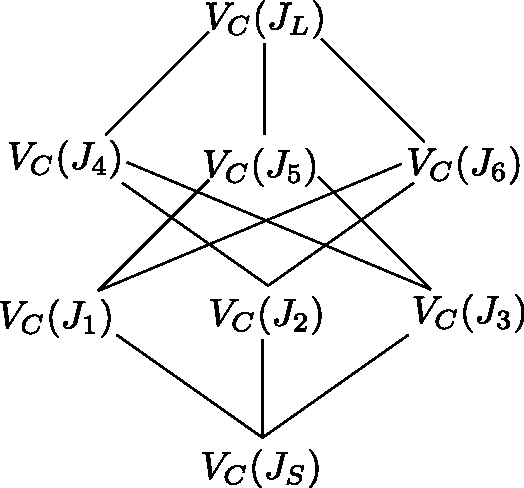
\includegraphics[width=0.8\textwidth]{interpolant_lattice.pdf}
\captionof{figure}{Interpolant lattice}
\label{Fig:int_lat}
% \begin{center}
% \end{figure}
\end{minipage}

It is easy to check  that all $V(J_I)$ satisfy the 3 conditions of
Def. \ref{def:int}. Note also that $V(J_S)$ is the smallest
interpolant, contained in every other interpolant. Likewise, $V(J_L)$
contains all other interpolants and it is the largest. The other
containment relationships are shown in the corresponding interpolant
lattice in Fig. \ref{Fig:int_lat}; i.e. $\Vc(J_1) \subset \Vc(J_5),
\Vc(J_1) \subset \Vc(J_6)$, and so on. 


 %% \begin{align*}
 %% & \Vc(J_1) \subset \Vc(J_5) ~~~~~~~~~~~~ \Vc(J_1) \subset \Vc(J_6) \\
 %% & \Vc(J_2) \subset \Vc(J_4) ~~~~~~~~~~~~ \Vc(J_2) \subset \Vc(J_6) \\
 %% & \Vc(J_3) \subset \Vc(J_4) ~~~~~~~~~~~~ \Vc(J_3) \subset \Vc(J_5)
 %% \end{align*}


}
\end{Example}



%% \begin{Example}
%% \label{example:jajb}
%% Consider the ideal $J_A$ from Example \ref{example:ja} and another
%% $J_B = \langle b,d,ec+e+c+1, ec \rangle$ with the variables of 
%% its generators partitioned as $B = \{e\}$ and $C = \{b,c,d\}$.
%% The intersection of varieties $\Vabc(J_A)$ and $\Vabc(J_B)$ is 
%% empty as,
%% \begin{align*}
%% \Vabc(J_A) &= \Fq^B \times \Vac(J_A)  \\
%% &= (abcde):\{ 01000,00010,01100,10010, \\
%% & ~~~~~~~~~~~~~~~~~~~~~~ 01001,00011,01101,10011 \} \\
%% \Vabc(J_B) &= \Fq^A \times \Vbc(J_B) \\
%% &= (abcde):\{00001,00100,10001,10100\}
%% \end{align*} 

%% Therefore, there must exist an interpolant satisfying the 
%% above three properties. 
%% \end{Example}


\begin{Theorem}
An ideal-interpolant $J_I$, and correspondingly the interpolant $\Vabc(J_I)$, as
given in Def. \ref{def:int}, always exists. 
\end{Theorem}

\begin{proof}
Consider the elimination ideal $J_I = J_A \cap \Fq[C]$. We show $J_I$ satisfies 
the three conditions for the interpolant. 

\par \noindent  \underline{Condition 1}: $\Vabc(J_I) \supseteq
\Vabc(J_A)$. This condition is trivially satisfied due  to
construction of elimination ideals. As $J_I \subseteq J_A$,
$\Vabc(J_I) \supseteq \Vabc(J_A)$.

%% In other words  any point in the $\Vabc(J_A)$ has
%% to satisfy all the polynomials in $J_I$ as $J_I$ is  a subset of
%% polynomials in $J_A$.  

\par \noindent \underline{Condition 2}: $\Vabc(J_I) \cap \Vabc(J_B) =
\emptyset$. This condition  can be equivalently stated as $\Vbc(J_I)
\cap \Vbc(J_B) = \emptyset$ as neither  $J_I$ nor $J_B$ contains any
variables from the set $A$. We prove this condition by
contradiction. Let's assume that there exists a
common point $(\mathbf{b},\mathbf{c})$ in $\Vbc(J_I)$ and $\Vbc(J_B)$.  
We know that the projection of the variety $Pr_A(\Vac(J_A))$ is equal
to the variety of the elimination ideal $\Vc(J_I)$, where $J_I=J_A
\cap \Fq[C]$, due to Lemma \ref{lemma:project}. 
 %% (as $J_A$ is radical). 
Therefore, the point $(\mathbf{c})$ in the variety of $J_I$ can be
extended to a point $(\mathbf{a},\mathbf{c})$ in the variety of
$J_A$. This implies that the ideals $J_A$ and $J_B$ vanish at 
($\mathbf{a},\mathbf{b},\mathbf{c}$). This is a contradiction to our
initial assumption that the intersection of the varieties of $J_A$ and
$J_B$ is empty.  Thus $J_I, J_B$ have no common zeros.

\par \noindent \underline{Condition 3}: The generators of $J_I$
contain only the $C$-variables. This condition is trivially satisfied
as $J_I$ is the elimination ideal obtained by  eliminating
$A$-variables in $J_A$. 
\end{proof}

The above theorem not only proves the existence of an interpolant, but
also gives a procedure to construct one: $J_I = J_A\cap\Fq[C]$. In
other words, compute a reduced Gr\"obner basis $G$ of $J_A$ w.r.t. an
elimination order $A> B > C$ and take $G_I = G \cap \Fq[C]$. Then
$G_I$ gives the generators for the ideal-interpolant $J_I$.

\begin{Example}
{\it 
The elimination ideal $J_I$ computed for $J_A$ from Example \ref{ex:main}
is $J_I = J_S = \langle cd,b+d+1 \rangle$ with variety
$\Vc(J_I)=(bcd):\{001,100,110\}$.  This variety over the variable set
$A$ and $C$ is $\Vac(J_I)=(abcd):\{0001,0100,0110, 1001,1100,1110\}$,
and it contains $\Vac(J_A)$. Moreover, $\Vabc(J_I)$ also has an empty
intersection with $\Vabc(J_B)$. 
}
\end{Example}

%The next theorem proves that this variety $\Vc(J_I)$ is also the
%smallest interpolant, $i.e.$ all other interpolants contain it. 

\begin{Theorem}
\label{thm:smallest}
The interpolant $\Vabc(J_S)$ corresponding to the ideal %-interpolant
$J_S = J_A \cap \Fq[C]$ is the smallest interpolant.
\end{Theorem}

\begin{proof} 
The proof is given in the appendix. 


%% Let $J_I \subseteq \Fq[C]$ be any another ideal-interpolant $\neq
%% J_S$. We show that $\Vc(J_S) \subseteq \Vc(J_I)$. For $\Vc(J_I)$
%% to be an interpolant it must satisfy 
%% \begin{align*}
%% \Vabc(J_A) \subseteq \Vabc(J_I)
%% \end{align*}
%% which is equivalent to 
%% \begin{align*}
%% I(\Vabc(J_A)) &\supseteq I(\Vabc(J_I)) \\
%% \implies J_A &\supseteq J_I  
%% \end{align*}
%% due to Theorem \ref{thm:strong-ns}.
%% %% as $J_I$ is radical so $I(\Vabc(J_I)) = J_I)$. 
%% As the generators of $J_I$ only contain polynomials in $C$-variables,
%% this relation also holds for the following
%% \begin{align*}
%% J_A \cap \Fq[C] &\supseteq J_I \\
%% \implies J_S &\supseteq J_I \\
%% \implies \Vc(J_S) &\subseteq \Vc(J_I).
%% \end{align*} 
\end{proof}

%After proving that the elimination ideal $J_A \cap \Fq[C]$ is the
%smallest interpolant, 
Now we discuss how the largest interpolant can be
computed. For this, we will make use of quotients of ideals. 

\begin{Definition}
\label{def:quo}
({Quotient of Ideals}) If $J_1$ and $J_2$ are ideals in a ring $R$,
then $J_1:J_2$ is the set 
%  \begin{equation}
  $\{f \in R \ |\ f\cdot g \in J_1, \forall g \in J_2\}$ %\nonumber
%  \end{equation}
and is called the {\bf ideal quotient} of $J_1$ by $J_2$.
\end{Definition}

We use ideal quotients to compute the complement of a variety. Given
an ideal $J' \subset R$ containing the vanishing polynomials, suppose
we need to find an ideal $J$ such that $V(J) = \Fq^n - V(J') = V(J_0)
- V(J')$, where ``$-$'' corresponds to the set difference
operation. Then $J = J_0 : J'$ (see Theorem III.2 and Corollary III.1
in \cite{xiaojun:hldvt2016} for a proof outline). Once again, the
Gr\"obner basis algorithm can be used to compute $J_0:J'$ 
\cite{ideals:book}.  

\begin{Theorem}
\label{thm:large}
Consider the elimination ideal $J'_L = J_B \cap \Fq[C]$. The
complement of the variety $\Vc(J'_L)$,  computed as $\Fq^C - \Vc(J'_L)$,
is the largest interpolant.
\end{Theorem}

\begin{proof} Proof is given in the appendix. 

%% We first prove that the interpolant computed by
%% complementing $\Vc(J'_L)$  as $\Fq^C - \Vc(J'_L)$ is indeed a valid
%% interpolant. As $J'_L$ is the elimination ideal computed from $J_B$,
%% $\Vbc(J'_L) \supseteq \Vbc(J_B)$. This in turn implies that the
%% complement of $V(J'_L)$ cannot intersect with $V(J_B)$ at any
%% point. This proves condition 2 for $\Fq^C - \Vc(J'_L)$ to be a
%% valid interpolant.  

%% For condition 1, we need to prove that
%% \begin{align*}
%% \Vac(J_A) \subseteq \Fq^A \times (\Fq^C - \Vc(J'_L))
%% \end{align*}
%% This can be restated as
%% \begin{align*}
%% \Vac(J_A) \cap \Fq^A \times \Vc(J'_L) = \emptyset
%% \end{align*}
%% Let us assume (by contradiction) that there exists a common point 
%% $(\mathbf{a},\mathbf{c})$ in $\Vac(J_A)$ and $\Fq^A \times
%% V_C(J'_L)$. As the projection $Pr_B(\Vbc(J_B))$ on the
%% $C$-variables is equal to  the variety of the elimination ideal
%% $\Vc(J'_L)$, a point $(\mathbf{c}) \in \Vc(J'_L)$ can be  extended to
%% some point $(\mathbf{b},\mathbf{c})$ in $\Vbc(J_B)$. This implies that
%% the point $(\mathbf{a},\mathbf{b},\mathbf{c})$ is a common point in
%% $\Vabc(J_A)$ and $\Vabc(J_B)$, which is a contradiction to our initial
%% assumption. Therefore condition 1 of Def. \ref{def:int} is satisfied
%% too and $\Fq^C - \Vc(J'_L)$ is indeed an interpolant. 

%% \par \noindent Next we prove that $\Fq^C - \Vc(J'_L)$ is the largest
%% interpolant. Consider an arbitrary ideal-interpolant $J_I$. We want to
%% prove $\Vc(J_I) \subseteq \Fq^C - \Vc(J'_L)$, or equivalently to prove
%% $\Vc(J_I) \cap \Vc(J'_L) = \emptyset$. Let us assume (by contradiction) 
%% that there exists a common point $(\mathbf{c})$ in $\Vc(J_I)$ and
%% $\Vc(J'_L)$. As $J'_L$ is the elimination ideal of $J_B$, this point
%% can be extended to some point $(\mathbf{b},\mathbf{c})$  
%% in $\Vbc(J_B)$. This in turn implies that $(\mathbf{b},\mathbf{c})$ is
%% a common point in  $\Vbc(J_B)$ and $\Fq^B \times \Vc(J_I)$. This is a
%% contradiction as an interpolant cannot intersect with the variety of
%% $J_B$. Hence, $\Fq^C - \Vc(J'_L)$ is the largest interpolant and it
%% contains all other interpolants.

\end{proof}

Let $J_L$ be the radical ideal corresponding to the largest
interpolant $\Vc(J_L) = \Fq^C - \Vc(J'_L)$. This ideal-interpolant
$J_L$ can be computed as $J_L = (J_{0,C}:J'_L)$, where $J_{0,C}$ is
ideal of vanishing polynomials in $C$-variables.  


\begin{Example}
{\it 
The ideal-interpolant $J_L = \langle bd + b + d + 1 \rangle$ in 
Example~\ref{ex:main} is computed as:
\begin{itemize}
	\item First compute the ideal $J'_L = J_B \cap \Fq[C]$ which results in 
	$J'_L = \langle b,d \rangle$.
	\item Then compute $J_L$ as $J_L = J_{0,C}: J'_L$ which results in
	$J_L = \langle bd + b + d + 1 \rangle$
\end{itemize}
The variety $V_C(J_L)=(bcd):\{001,011,100,101,110,111\}$ and it is the
largest interpolant for the given pair ($J_A,J_B$). 
}
\end{Example}

\begin{Lemma}
\label{noofinter}
The total number of interpolants for the pair ($J_A,J_B$) is
$2^{|SM(J_D)|}$, where $J_D = (J_L:J_S)$. 
\end{Lemma}

\begin{proof}
The proof is given in the appendix. 

%% The smallest and the largest interpolants are $\Vc(J_S)$ and $\Vc(J_L)$,
%% respectively. The set difference $\Vc(J_L) - \Vc(J_S)$ is also a
%% variety of some ideal $J_D$, which can be computed as
%% $J_D=(J_L:J_S)$. By selecting different subsets of $\Vc(J_D)$ and
%% adding them to $\Vc(J_S)$, we can generate all the 
%% interpolants. Consider, 
%% \begin{align*}
%% \label{eqn:pwsetjd}
%% \binom{|\Vc(J_D)|}{0} + \binom{|\Vc(J_D)|}{1} + \cdots + \binom{|\Vc(J_D)|}{|\Vc(J_D)|} = 2^{|\Vc(J_D)|}
%% \end{align*}
%% where the term $\binom{|\Vc(J_D)|}{0}$ denotes that no point is selected from $\Vc(J_D)$ and results in 
%% $\Vc(J_S)$ as the ideal-interpolant. On the other hand, the term $\binom{|\Vc(J_D)|}{|\Vc(J_D)|}$ is equivalent 
%% to selecting  all the points from $\Vc(J_D)$ and results in $J_L$ as 
%% the ideal-interpolant. So the number of interpolants is equal to
%% $2^{|\Vc(J_D)|}$. Theorem \ref{thm:count} further tells us that the 
%% cardinality of a variety of an ideal is equal to the number of
%% standard monomials of that ideal, therefore, number of interpolants $=
%% 2^{|SM(J_D)|}$.  

\end{proof}

\begin{Example}
\label{ex:jd}
{\it 
From Example~\ref{ex:main}
$J_L = \langle bd + b + d + 1 \rangle$ and $J_S = \langle cd, b + d+
1\rangle$. 
Computing $J_D = J_L : J_S$ gives $J_D = \langle
d+1,bc+b+c+1,c^2+c,b^2+b \rangle$, where the variety $\Vc(J_D)=\Vc(J_L)-\Vc(J_S)
=(bcd):\{011,101,111\}$. 

The standard monomials for $J_D$ are $SM(J_D) = \{1,b,c\}$. Therefore,
the total number of interpolants for the given pair ($J_A,J_B$) is
$2^{|\{1,b,c\}|}=2^3=8$. 
}
\end{Example}


\subsubsection{The structure of the interpolant lattice:} Note that
our results do provide some insights into the structure of the
interpolant lattice. Let $l = |SM(J_D)|$. Then, the height of the
interpolant lattice is $l + 1$, and the number of elements (interpolants) at each
level $i$ is $l \choose i$, $0\leq i \leq l$. Notice also that the size (height and
width) of the interpolant lattice is independent of the number of
variables in the set $C$, and depends only on $|SM(J_D)|$. 

%% Next we describe a procedure for enumerating all of these interpolants using the $SM(J_D)$.
%% Let's say there are $l$ standard monomials, $\{m_1,\dots,m_l\}$ in the set $SM(J_D)$. Consider
%% a polynomial $f_i$ constructed using the linear combination of $\{m_1,\dots,m_l\}$ as,
%% \begin{center}
%% $f_i = \lambda_1\cdot m_1 + \lambda_2\cdot m_2 +\cdots+ \lambda_l\cdot m_l$
%% \end{center} 
%% where each $\lambda_i \in \mathbb{F}_2$ $i.e.$ $\lambda_i \in \{0,1\}$.
%% There can be exactly $2^l$ unique polynomials obtained in this way.
%% We can then obtain all the ideal-interpolants $I_j$ as,
%% \begin{center}
%% $I_j = J_S\cdot(J_D + \langle f_i \rangle)$
%% \end{center}
%% where $\langle f_i \rangle$ is the ideal generated by the polynomial $f_i$.

\section{Experimental Results}
\label{sec:exp}

This section presents the results of using our implementation
(Algorithm~\ref{multimon}) for formal verification and equivalence
checking of circuits used in cryptography. We compare our results
against: i) F4-style reduction~\cite{pruss:tcad} which models the
reduction as Gaussian elimination on a coefficient matrix;   ii)
Parallelized approach for performing reductions on Galois field 
multipliers~\cite{cunxi:aspdac17};  and iii) PolyBori's \cite{polybori:2009}
%% that uses the conventional
reduction procedure with ZDDs as the
underlying data structure. For all tools and experiments, RTTO $>$ is
used for constraint representation. 
 The experiments are performed on a 3.5GHz
Intel Core\textsuperscript{TM} i7-4770K Quad-Core CPU with 32 GB of
RAM. 
% Experiments are conducted for verification of finite field
% multipliers and polynomial computation modules used as cryptography
% primitives. 
The data-path sizes {$k$} are selected according to
cryptography standards recommended by U.S. National Institute of
Standards and Technology (NIST). 
% Modular multiplication is an important computation used in cryptography. 
% We have performed experiments with two architectures for this multiplication, namely Mastrovito and Montgomery. 

\subsection{Mastrovito Multipliers}

Modular multiplication is an important computation used in
cryptography. A Mastrovito multiplier architecture can be employed for
performing this computation over the finite field of $2^k$ elements,
i.e. $\mathbb{F}_{2^k}$. Mastrovito multipliers compute $Z = A\times B \pmod{
  P(x)}$ where $P(x)$ is a given primitive polynomial for the datapath size
$k$. Here $A = \{a_0,a_1,\dots,a_{k-1}\}$, $B = \{b_0,b_1,\dots,b_{k-1}\}$ are the
two data operands, and
$Z = \{z_0,z_1,\dots,z_{k-1}\}$ is the output.
The product $A \times B$ is first computed using an array multiplier
architecture, and then the result is reduced modulo $P(x)$. 
% The following example demonstrates the Mastrovito multiplier
% computation~\cite{lv:tcad2013}. 

% \begin{Example}
% \label{exp1}
% {\it 
% Consider the finite field $\mathbb{F}_{2^4}$ where the operand size is 4. Let the inputs be:
% $A=a_0+a_1\cdot \alpha+a_2\cdot \alpha^2+a_3\cdot \alpha^3$ and
% $B=b_0+b_1\cdot \alpha+b_2\cdot \alpha^2+b_3\cdot \alpha^3$, and 
%  the primitive polynomial be $P(x)=x^4+x^3+1$ with $\alpha$ as its
%  root so that $P(\alpha) = 0$.  
%  % We have to perform the multiplication $Z =A\times B \pmod{ P(x) }$. 
% The constituent bits of $A$  and $B$ are $\{a_0, \dots, a_3\}$ and
% $\{b_0, \dots, b_3\}$ respectively, which are the primary inputs of
% the circuit. First, we perform the multiplication $A\cdot B$ as:

% %\vspace{-0.2in}

% \vspace{0.05in}

% {\small
% {\begin{tabular}{c c c c c c c c}
% %\vspace{-0.2in}
%   &   &   & $a_3$ & $a_2$ & $a_1$ & $a_0$  \\ 
%  $\times$&   &   & $b_3$ & $b_2$ & $b_1$ & $b_0$  \\ 
%  \hline
%  &   &   & $a_3\cdot b_0$ & $a_2 \cdot b_0$ & $a_1\cdot b_0$ & $a_0\cdot b_0$ \\
%  &  & $a_3\cdot b_1$ & $a_2\cdot b_1$ & $a_1 \cdot b_1$ & $a_0\cdot b_1$ &   \\
%  & $a_3\cdot b_2$ & $a_2\cdot b_2$ & $a_1\cdot b_2$ & $a_0\cdot b_2$ &  &   \\
%  $a_3\cdot b_3$ & $a_2\cdot b_3$ & $a_1\cdot b_3$ & $a_0\cdot b_3$ &  &  &   \\
%  \hline
%  $s_6$& $s_5$  & $s_4$  & $s_3$ & $s_2$  & $s_1$   & $s_0$ 
% % \vspace{-0.2in}
% \end{tabular}}
% }

% \vspace{0.05in}

% The result $S = s_0+s_1\cdot \alpha + s_2\cdot \alpha^2 + s_3\cdot
% \alpha^3 + s_4\cdot \alpha^4 + s_5\cdot \alpha^5 + s_6\cdot \alpha^6$,
% where, $s_0  =  a_0\cdot b_0, ~~s_1  =  a_0\cdot b_1 + a_1\cdot b_0,
% ~~s_2 = a_0\cdot b_2 + a_1\cdot b_1 + a_2\cdot b_0$, and so on. Here
% the multiply ``$\cdot$'' and add ``$+$'' operations are performed
% modulo 2, and hence implemented in a circuit using AND and XOR
% gates. As the coefficients are always reduced $\pmod 2$ in $\mathbb{F}_{2^k}$, there are no carry-chains
% in the design. Next, the result $S$ is reduced modulo the primitive
% polynomial $P(x) = x^4 + x^3 + 1$, as:
% % where the final output of the circuit is denoted by $G(x)  = g_3x^3
% % + g_2x^2 +g_1x + g_0$.  

% \vspace{0.05in}

% {\small
% {\begin{tabular}{|c c c c | l }
%   $s_3$   &$s_2$    &$s_1$   &$s_0$   &   \\
%  \hline
%  $s_4$    &$0$    &$0$   &$s_4$   &$s_4\cdot \alpha^4 \pmod{P(\alpha)} = s_4 \cdot (\alpha^3 + 1)$\\
%  $s_5$    &$0$    &$s_5$   &$s_5$     &$s_5\cdot \alpha^5 \pmod{P(\alpha)} = s_5\cdot (\alpha^3+ \alpha + 1)$\\
%  $s_6$    &$s_6$    &$s_6$   &$s_6$     &$s_6\cdot \alpha^6 \pmod{ P(\alpha)} = s_6\cdot( \alpha^3 + \alpha^2 + \alpha + 1)$\\
%  \hline
%  $z_3$    &$z_2$    &$z_1$   &$z_0$   &
%  \end{tabular}\par}
% }

% \vspace{0.05in}

% The primary output of the circuit is: $Z = \{z_0, \dots, z_3\}$,
% represented as $Z =  z_0 + z_1 \alpha + z_2
% \alpha^2 + z_3 \alpha^3$; where  $z_0=s_0+s_4+s_5+s_6; ~~z_1=s_1+s_5+s_6;
% ~~z_2=s_2+s_6; ~~z_3=s_3+s_4+s_5+s_6$. 
% }
% \end{Example}

\par Table~\ref{masmmsyn} provides the results for the reductions $z_i
\xrightarrow{G}_+ r_i$ for Mastrovito multipliers for each output bit
$z_i, 0\leq i \leq k-1$. The benchmarks are taken
from~\cite{lv:tcad2013} and optimized using ABC~\cite{ABCtool} with
the commands $resyn2$ and $dch$ as mentioned
in~\cite{cunxi:aspdac17}. Algorithm~\ref{multimon} reduces each output
bit independently of other bits. Therefore, we have presented the
results obtained by running our reduction algorithm both 
sequentially and in parallel for each output bit. Similarly, the results for
implementation in PolyBori are also presented for both cases. The
implementation presented in \cite{cunxi:aspdac17} is already
parallelized. We parallelized PolyBori and our implementation by
creating individual processes for  each output bit $z_i$ that has its
own set of variables and gate polynomials, $poly\_list$
(Algorithm~\ref{multimon}). The maximum number of parallel processes
is decided upon the memory usage of each process ($i.e.$ reducing one
bit) for our implementation and the total available memory. The larger
benchmarks are run with fewer parallel processes as they consume more
memory. 
% As ZDDs are more complex data structures compared to those used in~\cite{cunxi:aspdac17}, the upper limit of memory usage for each bit is set by our implementation. For instance, an individual process in the reduction of 283-bit multiplier can take upto $\sim 3\%$ of available memory as compared to $\sim 6\%$ in the case of 409-bit mulitplier. Therefore, we run the all the implementations with 20 parallel processes for 283-bit multiplier but only with 10 for 409-bit multiplier. 
\par In the table, the column \#T represents the number of parallel
processes. (S) and (P) refer to the cases when the experiments run
sequentially and in parallel for the output bits $z_i$, respectively.  

%%%%%%%%%%%%% Syn Mas Multipliers %%%%%%%%%%%%%%%%%%%

\begin{table}[ht]
\centering
%\caption{Synthesized Mastrovito Multipliers (Time in seconds, \# of nodes, \# of redundant monomials in $k$)  (K = $10^3$, M = $10^6$)}
\caption{Mastrovito Multipliers (Time in seconds);  $k$ = Datapath Size, \#Gates = No. of gates, \#T = No. of threads, Time-Out = 30 hrs, (P): Parallel Execution, (S): Sequential Execution, K = $10^3$, M = $10^6$, PB: PolyBori, ZR: Algorithm~\ref{multimon}}
\label{masmmsyn}
\begin{tabular}{| c | c || c | c | c | c | c | c | c |} \hline
%\multirow{2}{*}{\textbf{Input}} & \multirow{2}{*}{\textbf{Abstraction}} & \multicolumn{3}{ c |}{\textbf{ZDD reduction(ZR)}}  &  \multirow{2}{*}{\textbf{ZR improved}}\\ \cline{3-5}
% & &Building ZDDs&Reduction&Total&\\ \hline
\multirow{2}{*}{$\boldsymbol{k}$}&\multirow{2}{*}{\textbf{\#Gates}}&\multirow{2}{*}{\textbf{F4~\cite{pruss:tcad}}}& \multirow{2}{*}{\textbf{\#T}}&\multirow{2}{*}{\textbf{~\cite{cunxi:aspdac17}(P)}}& \multicolumn{2}{ c |}{\textbf{PB}}&\multicolumn{2}{ c |}{\textbf{ZR}}\\ \cline{6-9}
&&&&&\textbf{(P)}&\textbf{(S)}&\textbf{(P)}&\textbf{(S)} \\ \hline
64 &11.5K&1.3&20& 3.70&3.60& 2.21&0.73 &\textbf{0.27}\\ \hline 
% 96 &25.6K&&20& 11.66&10.25&6.92 &2.04 &\textbf{0.66}\\ \hline 
128 &46K&9.89&20&27.54 &23.99&16.76& 5.08 &\textbf{1.63}\\ \hline 
163 &73.5K&32.61&20& 55.96&48.67&33.72&  11.41&\textbf{3.11}\\ \hline 
233 &122K&86.30& 20&127.61&112.96 &77.23& 21.77&\textbf{3.63}\\ \hline
283 &193K&274.68& 20&253.05&227.77&157.45& 49.89&\textbf{11.41}\\ \hline
409 &386K&2,528.5& 10&716.80 &659.64&426.92& 163.52&\textbf{17.68}\\ \hline
571* &1.6M & TO &3 & 5,331&CR&CR&2,126.7& \textbf{566.4}\\ \hline
\end{tabular}
\end{table}
%\fi{}

%%%%%%%%%%%%%%%%%%%%%%%%%%%%%%%%%%%%%%%%%
\par The 571-bit multiplier could not be synthesized and mapped with
the given memory due to its large size. Therefore, we have provided
results for a structured (but unoptimized) 571-bit multiplier
benchmark. Our implementation outperforms the explicit approaches
of~\cite{pruss:tcad} and~\cite{cunxi:aspdac17} for Mastrovito
multipliers and also PolyBori. For the 571-bit multiplier, the
implementation of~\cite{pruss:tcad} does not finish for the given time
period of 30 hours and the PolyBori implementation crashes (CR).
The maximum memory consumption by ZDDs for Mastrovito multipliers
when GBR is performed sequentially varies from 131.6 MB for 64-bit
operands to 8.1 GB for 571-bit operands.

\par An interesting point to note in Table~\ref{masmmsyn} is that
our implementation takes less time when run
sequentially. There is a certain overhead involved when we declare
variables and build ZDDs for each gate of the circuit. In the case of
Mastrovito multiplier benchmarks, this overhead is substantially
greater than the reduction time for each output bit. Therefore, when
the output bits are reduced in parallel for these benchmarks, 
this overhead increases the overall run time.  
% For example, for the 64-bit multiplier the overhead is 22.09 ms (when running it sequentially), whereas the reduction time for most of the bits is $\sim 0.30$ ms. The sequential reduction time with these values is $22.09 + 64 (0.3) = 41.29$ ms. On the other hand, with 20 processes this time is approximately $(64/20)(22.09 + 0.3) = 71.65$ ms. 
% There are other factors involved too, $e.g.$ CUDD package maintains an internal cache that helps avoid duplicate computations. When performing reduction sequentially the operations involving fanouts can be stored in the cache and used during the reduction of different output bits. 
 
% {\bf Efficiency of our approach:} The efficiency of our approach is
% attributed to the implicit data-structure and the number of iterations
% ($while$ loop in Algorithm~\ref{singlemon}) that are saved while
% performing the GBR. Table~\ref{monomsave} shows  
% the number of explicit monomial cancellations
% that are {\it avoided in our approach} by exploiting the structure of the
% ZDDs, when applied for the GBR $z_i\xrightarrow{G}_+ r_i$ for
% verification of Mastrovito multipliers.  
% %The  number of monomials
% %that are generated and eventually gets canceled ($2\cdot(yd + y)$
% %expression in Eqn.~\ref{mteq})  due to operations being performed
% %$\pmod 2$ are exactly double the statistics provided in
% %Table~\ref{monomsave}. 

% \begin{table}[H]
% \centering
% \caption{Number of explicit monomial cancellations (MC) {\it saved} by using
%   our approach; K = $10^3$, M = $10^6$}
% \label{monomsave}
% \begin{tabular}{| c | c | c | c | c | c | c | c |} \hline
% $k=$& 64 &128 &163 &233 & 283& 409 & 571* \\ \hline
% MC& 22.8K&96.4K & 156.2K& 171.3K& 404.6K& 511.3K& 1.63M\\ \hline
% % & & & & & & & \\ \hline
% \end{tabular}
% \end{table}

\subsection{Montgomery Multipliers}{}
Exponentiation operations are often required in cryptosystems.  
For such applications, Montgomery architectures \cite{acar:1998} \cite{wu:2002}{}
% \cite{Barrett:1987} 
\cite{Knezevic:2008} are considered more efficient than Mastrovito multipliers
as they do not require explicit reduction modulo $P$ after each step.
% Montgomery multipliers perform fast modular multiplication without
% explicitly performing the reduction $\pmod{P}$. 
%They are more
%efficient than the Mastrovito multipliers when several modulo
%multiplications are required as in the case of exponentiation in
%cryptosystems. {}
Fig.~\ref{montfig} shows the structure of a Montgomery
multiplier. Each MR block computes $A\cdot B\cdot R^{-1}$, where $R$
is selected as a power of a base ($\alpha^{k}$) and $R^{-1}$ is the multiplicative 
inverse of $R$ in $\mathbb{F}_{2^k}$. As this operation cannot compute $A\cdot B$
directly, we need to pre-compute $A\cdot R$ and $B\cdot R$ as shown in the Fig.~\ref{montfig}. 
We denote the leftmost
two blocks as Block A (upper) and B (lower), the middle block as Block
C and the output block as Block D.
% We have presented results for GBR
%on both \textit{flattened} and \textit{hierarchical} netlists of these
% multipliers. 

\begin{figure}[ht]
  \centering
  %\def\svgwidth{340pt}
  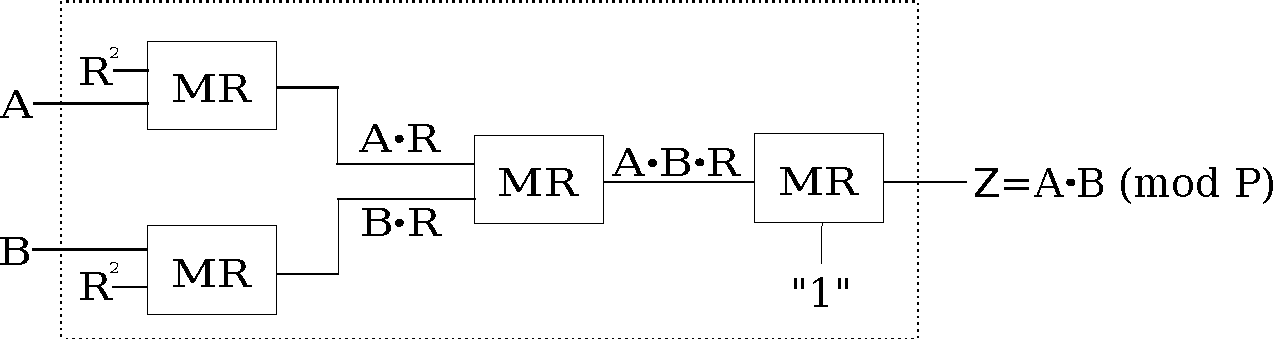
\includegraphics[scale=0.34]{figures/new_mmcircuit.pdf}
  \caption{Montgomery multiplication.}
  \label{montfig}
  \end{figure}



\par Table~\ref{montmmsyn} provides the results for GBR on flattened
(bit-blasted) and  optimized Montgomery multipliers for the sequential
and parallel executions of Algorithm
\ref{multimon}. The maximum  
memory consumption for sequential execution varies from 
66.7 MB for 64-bit operands to 11.3 GB for 571-bit operands.
% For most of these benchmarks the overhead is quite small than the
% reduction time for one bit except for the 233 and 409 bit
% multipliers. Therefore, we benefit from parallelizing the reduction
% process for these cases other than 283 and 409 bit multipliers.  
Our approach outperforms conventional explicit approaches except for
the case of 283 bit multiplier. 
% \textcolor{red}{Also, the reduction time for
% 283-bit circuit is more than 409-bit circuit. The reason is that 
% the bit-width of the multipliers is not the only factor controlling 
% the GBR time. The irreducible polynomial $P(x)$ also plays an
% important role in the designing of the multiplier and 
% consequently in the reduction as explained in \cite{cunxi:aspdac17}.} 

%%%%%%%%%%%%% Syn Mont Multipliers %%%%%%%%%%%%%%%%%%

\begin{table}[ht]
\centering
%\caption{Synthesized Mastrovito Multipliers (Time in seconds, \# of nodes, \# of redundant monomials in $k$)  (K = $10^3$, M = $10^6$)}
\caption{Montgomery Multipliers (Time in seconds); $k$ = Datapath Size, \#Gates = No. of gates, \#T = No. of threads, Time-Out = 30 hrs, (P): Parallel Execution, (S): Sequential Execution, K = $10^3$, M = $10^6$, PB: PolyBori, ZR: Algorithm~\ref{multimon}}
\label{montmmsyn}
\begin{tabular}{| c | c || c | c | c | c | c | c | c |} \hline
%\multirow{2}{*}{\textbf{Input}} & \multirow{2}{*}{\textbf{Abstraction}} & \multicolumn{3}{ c |}{\textbf{ZDD reduction(ZR)}}  &  \multirow{2}{*}{\textbf{ZR improved}}\\ \cline{3-5}
% & &Building ZDDs&Reduction&Total&\\ \hline
\multirow{2}{*}{$\boldsymbol{k}$}&\multirow{2}{*}{\textbf{\#Gates}}&\multirow{2}{*}{\textbf{F4~\cite{pruss:tcad}}}& \multirow{2}{*}{\textbf{\#T}}&\multirow{2}{*}{\textbf{~\cite{cunxi:aspdac17}(P)}}& \multicolumn{2}{ c |}{\textbf{PB}}&\multicolumn{2}{ c |}{\textbf{ZR}}\\ \cline{6-9}
&&&&&\textbf{(P)}&\textbf{(S)}&\textbf{(P)}&\textbf{(S)} \\ \hline
64 &9.5K&16.29&20&10.69&6.27&9.22& \textbf{3.75} & 8.37\\ \hline 
%96 &20.3K&&20&36.40&24.22& 22.0&\textbf{17.56} & 21.15\\ \hline 
128 &35K&621.90&20& 36.19&28.93&34.59&  \textbf{13.76}&24.73\\ \hline 
163 &56.5K&2,608.4&20&204.94 &167.73&335.2&  \textbf{141.68}&321.60\\ \hline 
233 &111K&385.92& 20&132.51& 119.77&99.36 &42.16&\textbf{31.88}\\ \hline
283 &165K&5,344& 20&\textbf{704.13}&1,194.2&2,078& 1,065.3&2,113\\ \hline
409 &340K&7,104& 10& 697.91&737.23& 722.1&303.91&\textbf{299.92}\\ \hline
571* &1.97M&TO&3&TO&CR&CR&\textbf{43,813}&99,042 \\ \hline
\end{tabular}
\end{table}
%\fi
%%%%%%%%%%%%%%%%%%%%%%%%%%%%%%%%%%%%%%%%%

\par Table \ref{montblockmm} presents the
statistics for Montgomery multipliers where the hierarchy of
Fig. \ref{montfig} for the blocks A, B, C, and D is made
available. The experiment first reduces the outputs of each individual
block modulo the gates of that block, and then reduces the primary
outputs modulo these four sets of remainders (ZDDs), thus exploiting
the hierarchy of these circuits. Table~\ref{montblockmm} shows the time
for reduction of each block and the time for reducing the primary
outputs across the four blocks. The  time for reducing the primary
outputs across the hierarchical blocks in case of the F4
implementation is $<$1 second, and is not explicitly mentioned in the
table. The row labeled \textit{Total} presents the sum of the
computation time of 
reduction across these levels, and the maximum of the time to reduce
each MR block (as the reductions for the four blocks are independent
of each other and are parallelized). These results again demonstrate
the efficiency of our approach against explicit approaches.
% The datapath sizes of these circuits correspond to
% NIST-specification in cryptography with $k = 163,\dots,571$ bits.

\begin{table}[ht]
\centering
% \caption{Montgomery Blocks(Time in seconds, Red. = time for reduction,
%   Coll. = time to reduce across the 4 levels.)}
\caption{Montgomery Blocks (Time in seconds); $k$ = Datapath Size, \#Gates = No. of gates, Time-Out = 30 hrs, 
Red. = time for reduction, Coll. = time to reduce across the 4 levels. 
% (P): Parallel Execution, (S): Sequential Execution, 
K = $10^3$, M = $10^6$, PB: PolyBori, ZR: Algorithm~\ref{multimon}}

\label{montblockmm}
\begin{tabular}{| c | c | c || c | c | c | c | c |} \hline
\multirow{2}{*}{$\boldsymbol{k}$}& \multirow{2}{*}{\textbf{\#Gates}}&\multirow{2}{*}{\textbf{Block}}& \multirow{2}{*}{\textbf{F4~\cite{pruss:tcad}}}  & \multicolumn{2}{ c |}{\textbf{PB}} &  \multicolumn{2}{ c |}{\textbf{ZR}} \\ \cline{5-8}
  & & & &Red. & Coll.  &Red. & Coll.  \\ \hline
\multirow{4}{*}{163} &33K &Block A & 25& 12 &\multirow{4}{*}{16} & 1 & \multirow{4}{*}{18}\\  \cline{2-5} \cline{7-7}
 & 33K&Block B &25 & 12 & & 1  &  \\  \cline{2-5} \cline{7-7}
 &85K&Block C &73 & 18 &&  7 &  \\  \cline{2-5} \cline{7-7}
 &32K&Block D &24 & 12 & & 1 & \\ \cline{2-8}
 &\multicolumn{2}{ c ||}{\textbf{Total}} & 73  &   \multicolumn{2}{ c |}{34} & \multicolumn{2}{ c |}{\textbf{25}}\\ \noalign{\hrule height 1.5pt}
\multirow{4}{*}{233}&55K&Block A  &142  & 32 & \multirow{4}{*}{5} & 0.14 & \multirow{4}{*}{4}\\  \cline{2-5} \cline{7-7}
 &55K& Block B &141 & 33 && 0.14  &  \\  \cline{2-5} \cline{7-7}
 &163K&Block C &408 & 34 & & 2.1  &  \\  \cline{2-5} \cline{7-7}
 &54K&Block D & 140& 32 && 0.13 & \\ \cline{2-8}
&\multicolumn{2}{ c ||}{\textbf{Total}}& 408  &   \multicolumn{2}{ c |}{39} & \multicolumn{2}{ c |}{\textbf{6.1}}\\ \noalign{\hrule height 1.5pt}
\multirow{4}{*}{283}&82K&Block A & 330 & 79 & \multirow{4}{*}{26} &24 & \multirow{4}{*}{90}\\  \cline{2-5} \cline{7-7}
&82K & Block B &329 & 78 && 23  &  \\  \cline{2-5} \cline{7-7}
&241K &Block C &883 & 173 &&  118 &  \\  \cline{2-5} \cline{7-7}
&81K &Block D &321 & 80 && 23 & \\ \cline{2-8}
&\multicolumn{2}{ c ||}{\textbf{Total}} & 883  &   \multicolumn{2}{ c |}{\textbf{199}} & \multicolumn{2}{ c |}{208}\\ \noalign{\hrule height 1.5pt}
\multirow{4}{*}{409}&168K&Block A & 1,322 & 177&\multirow{4}{*}{28} & 0.57 & \multirow{4}{*}{29}\\ \cline{2-5} \cline{7-7}
& 168K& Block B &1,335 &  175 &&  0.57 &  \\ \cline{2-5} \cline{7-7}
& 502K&Block C &4,471 & 192 &&  14 &  \\  \cline{2-5} \cline{7-7}
&168K &Block D &1,338 & 176 && 0.56 & \\ \cline{2-8}
&\multicolumn{2}{ c ||}{\textbf{Total}} & 4,471  &   \multicolumn{2}{ c |}{220} & \multicolumn{2}{ c |}{\textbf{43}}\\ \noalign{\hrule height 1.5pt}
\multirow{4}{*}{571}&330K&Block A &5,371 & 769 & \multirow{4}{*}{1,341} &321  & \multirow{4}{*}{1,412}\\  \cline{2-5} \cline{7-7}
&330K & Block B &5,421 & 747 && 332  &  \\ \cline{2-5} \cline{7-7}
 &980K&Block C &37,804 & 3,605 &&  3026 &  \\  \cline{2-5} \cline{7-7}
 &328K&Block D &5,539 & 751 && 338 & \\ \cline{2-8}
&\multicolumn{2}{ c ||}{\textbf{Total}}& 37,804  &   \multicolumn{2}{ c |}{4,946} & \multicolumn{2}{ c |}{\textbf{4,438}}\\ \noalign{\hrule height 1.5pt}


\end{tabular}
\end{table}


{\bf Equivalence Checking:} As a result of the GBR
$z_i\xrightarrow{G}_+ r_i$, the function implemented by each output
bit $z_i$ of the circuit is represented as a reduced, canonical,
Boolean polynomial in terms of the primary inputs, and by using a ZDD.
Thus the equivalence of such vastly different arithmetic circuit
implementations (Mastrovito vs Montgomery) can be verified by testing
for the equality (isomorphism) of the corresponding ZDD graphs. 


 %%%%%%%%% Point Addition Block D%%%%%%%%%%%%%%%%%%%%%%%%
\subsection{Point Addition over Elliptic Curves}
Point addition is an important operation required for the task of encryption, decryption 
and authentication in Elliptic Curve Cryptography (ECC). 
Modern approaches represent the points in projective
coordinate systems, {\it e.g.}, the L$\acute{o}$pez-Dahab (LD) projective coordinate \cite{eccld}, due to which the point addition 
operation can be implemented as polynomials in the field. 

\begin{Example}
{\it Consider point addition in L$\acute{o}$pez-Dahab (LD) projective coordinate. Given an elliptic curve: $Y^2 + XYZ = X^3Z + aX^2Z^2 + bZ^4$ over $\mathbb{F}_{2^k}$, where $X,Y,Z$ are $k$-bit vectors that are elements in $\mathbb{F}_{2^k}$ and similarly, $a, b$ are constants from the field. We represent point addition over the elliptic curve as ($X_3$, $Y_3$, $Z_3$) = ($X_1$, $Y_1$, $Z_1$) + ($X_2$, $Y_2$, $1$).  Then $X_3$, $Y_3$, $Z_3$ can be computed as follows:} 
\begin{align*}
&A = Y_2 \cdot Z_1^2 + Y_1  &&B = X_2 \cdot Z_1 + X_1 \\
&C = Z_1 \cdot B  &&D = B^2 \cdot(C + a Z_1^2) \\
&Z_3 = C^2 && E = A \cdot C  \\
&X_3 = A^2 + D + E &&F = X_3 + X_2 \cdot Z_3 \\
&G = X_3 + Y_2\cdot Z_3 && Y_3 = E\cdot F + Z_3 \cdot G
\end{align*}
\end{Example}
Each of the polynomials in the above design are implemented as a
(gate-level) logic block and are interconnected to obtain final
outputs $X_3,Y_3$ and $Z_3$. 

\begin{table}[ht]
\centering
\caption{Point Addition Circuits (Time in seconds); $k$ = Datapath Size, \#Gates = No. of gates, Time-Out = 30 hrs, K = $10^3$, M = $10^6$,
PB: PolyBori, ZR: Algorithm~\ref{multimon}}
\label{pointadd}
\begin{tabular}{| c | c || c | c | c |} \hline
$\boldsymbol{k}$&\textbf{\#Gates}&\textbf{F4~\cite{pruss:tcad}}&\textbf{PB}&\textbf{ZR} \\ \hline
64&15.3K&1.78&3.32&\textbf{0.72} \\ \hline
128&64K&40.55&27.41&\textbf{6.03} \\ \hline
163&104K&130.24&57.57&\textbf{13.13} \\ \hline
233&139K&335.60&106.85&\textbf{19.62} \\ \hline
283&281K&1,787.96&273.53& \textbf{64.48}\\ \hline
409&423K&5,077.50&578.15& \textbf{115.20}\\ \hline
571&1.14M&48,162.29&CR&\textbf{725.95} \\ \hline
\end{tabular}
\end{table}

The word-level abstraction approach in~\cite{pruss:tcad} presents the
results for extracting  the above representation for each of
$A,B,\dots, X_3,Y_3,Z_3$ blocks. It first performs a bit-level
reduction for every output of each block (GBR $z_i\xrightarrow{G}_+
r_i$), and then a  bit-to-word substitution to derive an input-output
word-level representation for the circuit. Table~\ref{pointadd} shows
the comparison of the time required for bit-level reduction of outputs
$d_i$ of the block $D= B^2\cdot(C + aZ_1^2)$ as done
in~\cite{pruss:tcad} against our implementation. (Bit-level
reductions for other blocks take much less time than that for block
D.) This result demonstrates that our bit-level GBR implementation
is in many cases orders of magnitude faster than the F4-style
reduction of \cite{pruss:tcad}. Therefore our approach can replace the
F4-style bit-level GBR of \cite{pruss:tcad} and improve the overall
process of word-level abstraction of datapath designs.   

\subsection{Equivalence Checking of Sequential Galois Field Multipliers}
The designs discussed so far are combinational implementations of
polynomial computations of finite filed circuits. These designs use
the standard basis representation $\{1,\alpha,\alpha^2, \dots,
\alpha^{k-1}\}$ to model a $k$-bit data-word $Z$ in terms of its
constituent bits as $Z = z_0 + z_1 \alpha + z_2 \alpha^2 \cdots +
z_{k-1} \alpha^{k-1}$, with $\alpha$ being the primitive element for
that field $\mathbb{F}_{2^k}$. 

\par 
%The size of the multipliers presented in the above sections
%become prohibitively large as $k$ increases.  
There exists sequential
multipliers where $k$-bit inputs are loaded into $k$-bit registers,
and the $k$-bit result is available  after $k$ clock-cycle execution
of the machine. These multipliers use a {\it normal basis}
$\{\beta,\beta^{2},\beta^{4},\dots,\beta^{2^{k-1}}\}$ to  represent a
$k$-bit data-word $S$ in terms of its constituent bits as $S =
s_0\beta + s_1\beta^{2} + s_2\beta^{4} \cdots s_{k-1}\beta^{2^{k-1}}$,
with $\beta$ being the normal element. The relation between $\alpha$
and $\beta$ can be used to represent  the bits $z_i$ and $s_j$ in
terms of each other.  

% \par The Normal basis are more efficient when performing multiplication and 
% exponentiations. The exponentiation operation can be achieved by simple cyclic-shift of the input bits. 
% As multiplication is more complex than exponentiation, it is performed by constructing a binary-valued $\lambda$-matrix $M$.
% %and then performing $A\times M \times B^T$ for inputs $A$ and $B$. 
% If the  matrix $M$ satisfies the property that the number non-zero elements is $2k-1$ (for data-path size $k$), then the
% normal basis is called an optimal normal basis (ONB). ONB is desirable for the construction
% of finite field circuits.  

\par We perform equivalence checking between two different
architectures of {\it sequential multipliers with parallel output
  (SMPO)}, the Agnew-SMPO (AG-SMPO) by
G.B. Agnew~\cite{agnew1991implementation} and the RH-SMPO by
Reyhani-Masoleh and Hasan~\cite{RHmulti}. 
% The values in the registers
% for all intermediate states  in these multipliers are different
% because they are based on two different mathematical principles.
% However, the final state of the output registers (i.e. after $k$ clock
% cycles) is the same as it is the result of the multiplication. 
In order to perform equivalence checking, the circuits are unrolled
over $k$ time frames, and the GBR $s_i \xrightarrow{G}_+ r_i$ 
is performed to obtain a canonical $r_i$ ($G$ is the set of
polynomials for the unrolled circuit under RTTO). The ZDDs for
respective $r_i$'s (for AG-SMPO and RH-SMPO) are compared to perform
equivalence check.    

% \par The authors in \cite{xiaojun:date15}\cite{xiaojun:phd} present an implicit unrolling approach for 
% sequential multipliers to derive a canonical word-level input-output relation. They present results for 
% two architectures of {\it sequential multipliers with parallel output (SMPO)} based on different 
% mathematical principles, the Agnew-SMPO (AG-SMPO) by G.B. Agnew~\cite{agnew1991implementation}
% and the RH-SMPO by Reyhani-Masoleh and Hasan~\cite{RHmulti}. 

%\par We perform the GBR $s_i \xrightarrow{G}_+ r_i$ for each output bit $s_i$ of the $k$-cycle unrolled 
% multipliers to obtain a canonical $r_i$. The $r_i$ can then be used to perform an equivalence check between the
% two architectures. 
Tables \ref{rhsmpo} and \ref{agsmpo} present the run-time of our
implementation for performing these reductions on RH-SMPO and AG-SMPO
architectures respectively, when compared with the approach presented
in \cite{pruss:tcad} and PolyBori. 
%Although normal bases exist for every $k$, optimal normal bases (ONB)
%do not. There are also different types of ONB. The values of $k$ in
%the tables correspond to Type-II ONB. For more details and a list of
%ONB field size, reader can refer to~\cite{gao:phd_normal_basis}. 
The results show that our implementation is about an order of
magnitude faster than PolyBori and multiple orders of magnitude faster
than the  explicit approach of~\cite{pruss:tcad}.
% The bit-widths in table are
% such that the corresponding normal basis are ONB. Our verification technique is multiple orders of magnitude faster than 
% that of~\cite{pruss:tcad} and an order of magnitude faster than the PolyBori.

\begin{table}[ht]
\centering
\caption{RH-SMPO Multipliers (Time in seconds); $k$ = Datapath Size, \#Gates = No. of gates, Time-Out = 30 hrs, K = $10^3$,
PB: PolyBori, ZR: Algorithm~\ref{multimon}}
\label{rhsmpo}
\begin{tabular}{| c | c | c | c | c | c | c | c | c |} \hline
$\boldsymbol{k=}$&65&81&89&131&173&233&281&410 \\ \hline
\textbf{\#Gates} & 13.6K&21.4K & 25.9K& 55.9K &96.5K&177K&258K&546K\\ \hhline{|=|=|=|=|=|=|=|=|=|}
\textbf{F4\cite{pruss:tcad}} &9.02 &26.65 & 42.46&294.7&874.3&3,404&7,328&23,610 \\ \hline
% \textbf{F4\cite{pruss:tcad}}   & 8.56&22.2 & 37.1&259.5&838.5&3,009&7566&23,610 \\ \hline %with bogus primitive polynomial
\textbf{PB}  &3.65 &6.07 & 7.42&28.22 &47.16&116.63&199.32&637.69\\ \hline
\textbf{ZR}  & \textbf{0.42}& \textbf{0.80}&\textbf{1.01} & \textbf{3.03}&\textbf{3.53}&
\textbf{8.12}&\textbf{13.27}&\textbf{52.09}\\ \hline
\end{tabular}
\end{table}

\begin{table}[ht]
\centering
\caption{AG-SMPO Multipliers (Time in seconds); $k$ = Datapath Size, \#Gates = No. of gates, Time-Out = 30 hrs, K = $10^3$,
PB: PolyBori, ZR: Algorithm~\ref{multimon}}
\label{agsmpo}
\begin{tabular}{| c | c | c | c | c | c | c | c | c |} \hline
$\boldsymbol{k=}$&65&81&89&131&173&233&281&410 \\ \hline
\textbf{\#Gates} &12.5K & 19.5K&23.6K&51.2K&89.4K&162K&236K&503K \\ \hhline{|=|=|=|=|=|=|=|=|=|}
\textbf{F4\cite{pruss:tcad}} &8.34 &20.46 &33.2&221.4&754.1&2,655&5,569&21,938\\ \hline
% \textbf{F4\cite{pruss:tcad}}  & 8.15& 19.18&29.1 &200.9&665.7&2,387&6,516&21,938 \\ \hline %with bogus primitive polynomial
\textbf{PB} &3.11 & 6.82& 9.21& 20.15&44.37&107.12&187.77&578.61\\ \hline
\textbf{ZR} &\textbf{0.44} &\textbf{0.77} &\textbf{0.91}& \textbf{2.51}&\textbf{3.39}&
\textbf{7.8}&\textbf{12.63}&\textbf{43.78}\\ \hline
\end{tabular}
\end{table}

% \begin{table}[H]
% \centering
% \caption{RH-SMPO Multipliers; $k$ = Datapath Size, \#Gates = No. of gates, Time-Out = 30 hrs, K = $10^3$,
% PB: PolyBori, ZR: Algorithm~\ref{multimon}}
% \label{rhsmpo}
% \begin{tabular}{| c | c | c | c | c | c | c | c | c | c | c |} \hline
% $\boldsymbol{k}$&33&51&65&81&89&131&173&233&281&410 \\ \hline
% \#Gates & 3.5K&8.5K & 13.6K&21.4K & 25.9K& 55.9K &96.5K&177K&258K&546K\\ \hhline{|=|=|=|=|=|=|=|=|=|=|=|}
% \cite{pruss:tcad} & 0.56& 3.3&9.02 &26.65 & 42.46&294.7&874.3&3,404&7,328& \\ \hline
% \cite{pruss:tcad} &0.88 &3.3 & 8.56&22.2 & 37.1&259.5&838.5&3,009&7566&23,610 \\ \hline %with bogus primitive polynomial
% PB &0.58 &1.96 &3.65 &6.07 & 7.42&28.22 &47.16&116.63&199.32&637.69\\ \hline
% ZR &\textbf{0.10} & \textbf{0.28}& \textbf{0.42}& \textbf{0.80}&\textbf{1.01} & \textbf{3.03}&\textbf{3.53}&
% \textbf{8.12}&\textbf{13.27}&\textbf{52.09}\\ \hline
% \end{tabular}
% \end{table}

% \begin{table}[H]
% \centering
% \caption{AG-SMPO Multipliers; $k$ = Datapath Size, \#Gates = No. of gates, Time-Out = 30 hrs, K = $10^3$,
% PB: PolyBori, ZR: Algorithm~\ref{multimon}}
% \label{agsmpo}
% \begin{tabular}{| c | c | c | c | c | c | c | c | c | c | c |} \hline
% $\boldsymbol{k}$&33&51&65&81&89&131&173&233&281&410 \\ \hline
% \#Gates &3.2K&7.7K&12.5K & 19.5K&23.6K&51.2K&89.4K&162K&236K&503K \\ \hhline{|=|=|=|=|=|=|=|=|=|=|=|}
% \cite{pruss:tcad} & 0.48& 2.78&8.34 &20.46 &33.2&221.4&754.1&2,655&5,569&\\ \hline
% \cite{pruss:tcad} &0.48 &2.76 & 8.15& 19.18&29.1 &200.9&665.7&2,387&6,516&21,938 \\ \hline %with bogus primitive polynomial
% PB & 0.52& 1.74&3.11 & 6.82& 9.21& 20.15&44.37&107.12&187.77&578.61\\ \hline
% ZR & \textbf{0.07}&\textbf{0.24} &\textbf{0.44} &\textbf{0.77} &\textbf{0.91}& \textbf{2.51}&\textbf{3.39}&
% \textbf{7.8}&\textbf{12.63}&\textbf{43.78}\\ \hline
% \end{tabular}
% \end{table}

% \begin{Example}
% {\it Consider a 3-bit RH-SMPO multiplier with output bits $\{r_2,r_1,r_0\}$ and input bits $\{p_2,p_1,p_0\}\{q_2,q_1,q_0\}$. 
% The multiplier performs the operation $R=P\cdot Q$, where $R=r_0\cdot \beta + r_1\cdot \beta^2 + r_2\cdot \beta^4$, 
% $P=p_0\cdot \beta + p_1\cdot \beta^2 + p_2\cdot \beta^4$ and $Q=q_0\cdot \beta +q_1\cdot \beta^2 + q_2\cdot \beta^4$. 
% Also consider a Mastrovito multiplier performing the operation $Z=A\cdot B$ with $Z=z_0\cdot  + z_1 \alpha + z_2\cdot \alpha^2$,
%  $A=a_0\cdot  + a_1 \alpha + a_2\cdot \alpha^2$ and $B=b_0  + b_1\cdot \alpha + b_2\cdot \alpha^2$ where $\{z_2,z_1,z_0\}$ and 
%  $\{a_2,a_1,a_0,b_2,b_1,b_0\}$ being the output and input bits respectively. The normal element $\beta$ in terms of standard basis 
%  element is $\beta = \alpha^3$. The primitive polynomial used in the design of Mastrovito multiplier is $P=X^3+X+1$ and $\alpha$ is the 
%  root of this polynomial.
%  \par The RH-SMPO multiplier output $R$ can be written in the notations of standard basis 
%  as $R = r_0\cdot \alpha^3 + r_1\cdot \alpha^6 + r_2\cdot \alpha^{12} = (r_0 + r_1 + r_2) + (r_0 + r_2)\cdot \alpha + (r_1 + r_2)\cdot \alpha^2$ using $\beta = \alpha^3$ and $\alpha^3 = \alpha +1$. Similarly, $P = (p_0 + p_1 + p_2) + (p_0 + p_2)\cdot \alpha + (p_1 + p_2)\cdot \alpha^2$ and $Q = (q_0 + q_1 + q_2) + (q_0 + q_2)\cdot \alpha + (q_1 + q_2)\cdot \alpha^2$. Therefore, }
% \begin{align*}
% & z_0 = r_0 + r_1 + r_2; ~~ z_1 = r_0 + r_2; ~~ z_2 = r_1 + r_2; \\
% & a_0 = p_0 + p_1 + p_2; ~~ a_1 = p_0 + p_2; ~~ a_2 = p_1 + p_2; \\
% & b_0 = q_0 + q_1 + q_2; ~~ b_1 = q_0 + q_2; ~~ b_2 = q_1 + q_2;
% \end{align*}
% {\it Solving for $p_i$ and $q_i$ in terms of $a_i$ and $b_i$ respectively,}
% \begin{align*}
% & p_0 = a_0 + a_2; ~~ p_1 = a_0 + a_1; ~~ p_2 = a_0 + a_1 + a_2; \\
% & q_0 = b_0 + b_2; ~~ q_1 = b_0 + b_1; ~~ q_2 = b_0 + b_1 + b_2;
% \end{align*}
% {\it Performing a bit-level reduction on $r_0,r_1$ and $r_2$ results in the following remainders,}
% \begin{align*}
% & r_0 = p_1\cdot q_0 + p_0\cdot q_1 + p_2\cdot q_1 + p_1\cdot q_2 + p_2\cdot q_2 \\
% & r_1 = p_0\cdot q_0 + p_2\cdot q_0 + p_2\cdot q_1 + p_0\cdot q_2 + p_1\cdot q_2 \\
% & r_2 = p_1\cdot q_0 + p_2\cdot q_0 + p_0\cdot q_1 + p_1\cdot q_1 + p_0\cdot q_2
% \end{align*}
% {\it Using $z_0 = r_0 + r_1 + r_2$, we get $z_0 = p_0\cdot q_0 + p_1\cdot q_1 + p_2\cdot q_2$. 
% Substituting $\{p_i,q_i\}$ in terms of $\{a_i,b_i\}$ results in $z_0 = a_0\cdot b_0 + a_1\cdot b_2 + a_2\cdot b_1$,
% which is also the remainder if we reduce the $z_0$ bit of the Mastrovito multiplier 
% modulo the polynomials of the gates of the circuit.
% }

% \end{Example}

% \begin{table}[H]
% \centering
% \caption{RH-SMPO Multipliers; k = Datapath Size, \#Gates = No. of gates, Time-Out = 30 hrs, K = $10^3$}
% \label{rhsmpo}
% \begin{tabular}{| c | c | c | c | c | c | c |} \hline
% \textbf{k}&33&51&65&81&89&99 \\ \hline
% \#Gates & 3.5K&8.5K & 13.6K&21.4K & 25.9K& 32K\\ \hline
% \cite{xiaojun:date15} & 112.6& 1,129&5,243 &20,724 &36,096 &67,021 \\ \hline
% PB & 0.59& 2.02&3.10 &5.99 &7.72 &13.26 \\ \hline
% ZR &\textbf{0.10} & \textbf{0.26}& \textbf{0.48}& \textbf{0.84}&\textbf{1.08} & \textbf{1.48}\\ \hline
% \end{tabular}
% \end{table}

% \begin{table}[H]
% \centering
% \caption{AG-SMPO Multipliers; k = Datapath Size, \#Gates = No. of gates, Time-Out = 30 hrs, K = $10^3$}
% \label{agsmpo}
% \begin{tabular}{| c | c | c | c | c | c |} \hline
% \textbf{k}&36&66&82&89&100 \\ \hline
% \#Gates &3.8K&13K&20K & 23.6K&29.8K \\ \hline
% \cite{xiaojun:date15} & 113& 3,673& 15,117& 28,986& 50,692\\ \hline
% PB &0.48 & 2.84& 6.93&7.29 & 9.91 \\ \hline
% ZR & \textbf{0.10}&\textbf{0.46} &\textbf{0.76} &\textbf{0.95} &\textbf{1.30} \\ \hline
% \end{tabular}
% \end{table}
\subsection{Limitations of our approach: Integer arithmetic circuits}
% \par {\bf Integer Multiplication:} When performing reduction on
% integer multiplication benchmarks, a large number of non-linear  %
% monomials are generated that can be canceled early in the reduction
% process by employing a word-level approach unlike  % our bit-level
% reduction approach.  % The polynomial algebra model is not suitable
% for random logic (synthesized) circuits, where AIG-based reduction
% makes verification efficient. This model is beneficial for custom
% designed arithmetic circuits, where AIGs/SAT fail. 
The GBR approach presented in the previous section, although
applicable to integer arithmetic circuits, is not computationally
feasible for their verification. 
%The logical cones of output variables in integer
%arithmetic circuits have a lot of logic sharing (common subexpressions) and generate a
%large number of non-linear terms. 
We evaluated  our technique on integer arithmetic multiplier
circuits, which showed an  exponential increase in verification time
$w.r.t.$ the circuit size. This is because our approach reduces 
each primary output bit independently, and does not consider the logic
sharing among different primary outputs. As a result, a large number
of monomials are generated during reduction that are common to 
multiple primary outputs. This effect of logic sharing cannot be
exploited in GBR when each primary output bit is reduced
independently. 
For example, the ZDD-based bit-level GBR for a 7x7 integer
multiplier reveals that when reducing the $z_{13}$ bit (MSB) and
the $z_{12}$ bit independently, the maximum number of monomials
encountered ($i.e.$ during $z_{13} \xrightarrow{G}_+ r_{13}$ and
$z_{12} \xrightarrow{G}_+ r_{12}$) are 429,889 and 897,955,
respectively.  However, the modulo-2 sum (XOR) of these ZDDs contains
only 789,604 monomials  (during the modulo-2 sum common monomials
cancel out) as opposed to 1,327,844 (= 429,889 + 897,955).
A word-level reduction approach (such as those of
\cite{ciesielski:dac2015} and \cite{rolf:date16}) may cancel such
common non-linear terms early in the reduction process and avoid
intermediate blow-up in the number of monomials. This is shown below.
%This  
%implies that even an implicit data-structure
%cannot accommodate the large number of non-linear terms
%that result in intermediate expression swell.
% Performing a detailed analysis reveals that for
% integer arithmetic datapath circuits, a bit-level reduction is {\it
%   not sufficient} for verification efficiency, and a word-level
% approach is required. %, such as the ones presented in 
\begin{figure}[hbt]
\centering
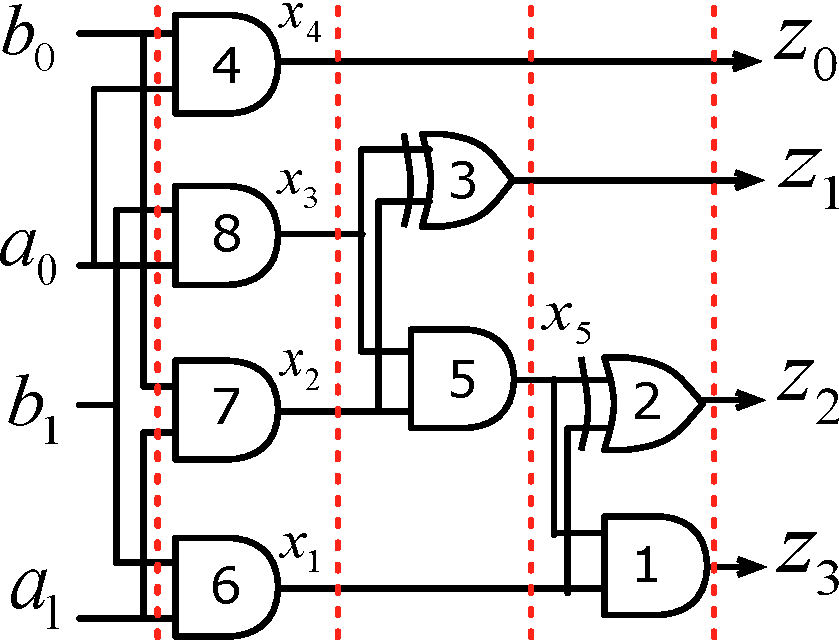
\includegraphics[scale=0.4]{figures/2-bit-mult_flipped.pdf}
\caption{Integer multiplier circuit}
\label{intmult}
\end{figure}
%\textcolor{red}{ A better 
%approach would be to perform a word-level reduction similar to
%the following example.
%}
Consider the integer multiplier circuit given in
  Fig. \ref{intmult}. A 
word-level approach would model the output word as 
$Z = z_0 + 2z_1 + 4 z_2 + 8 z_3$, and perform the reduction
$Z\xrightarrow{G}_+R$ across the reverse topological levels (RTTO) 
depicted in the figure. The polynomials of the circuit are:
\begin{align*}
z_0 &= x_4 \\ 
z_1 &= x_2 + x_3 - 2x_2x_3\\
z_2 &= x_1 + x_5 - 2 x_1 x_5 
    = x_1 + x_2x_3 - 2x_1x_2x_3\\
z_3 &= x_1x_5 = x_1x_2x_3
\end{align*}
Here $+$ denotes addition over integers. The reduction
of the word-level expression $8z_3 + 4z_2+2z_1+z_0$ in $Z$ cancels out the
common nonlinear monomials to control intermediate monomial explosion:
\begin{align*}
Z &= 8z_3 + 4z_2+2z_1+z_0\\
  &=\underline{8x_1x_2x_3} + (4x_1 + \underbrace{4x_2x_3} -
  \underline{8x_1x_2x_3})\\
  & + (2x_2+2x_3-\underbrace{4x_2x_3}_{}) + x_4\\
  &=4x_1 + 2x_2 + 2x_3 + x_4
\end{align*}
A purely
bit-level GBR approach is thus not suitable for integer arithmetic
circuits. However, this is not a limitation of our algorithms and
implementations, but rather an issue of the capability of bit-level
versus word-level models. Integrating the implicit data structure with
a word-level representation may yield better results for
such applications.
%% This modulo-2 sum indicates that reducing all the outputs simultaneously results 
%% in monomials that can cancel each other. Therefore, verification of integer multipliers require a word-level
%% decision procedure, as given in \cite{ciesielski:dac2015}
%% \cite{rolf:date16}, that accounts for the cancellation of these
%% monomials across multiple bits in one word-level expression whereas a pure bit-level reduction
%% is not sufficient to solve the problem. The experiment suggests that for integer 
%% arithmetic multipliers, 



% The reduction times for small integer arithmetic array multipliers are
% presented in Table \ref{intmm}. There is an 8x increase in time when
% moving from $n-1$ datapath size to $n$-bits, which is an exponential
% increase. Performing detailed analysis of a 7x7 multiplier reveals
% that, when reducing the $z_{13}$ bit (MSB) and $z_{12}$ bit of this
% circuit, the maximum number of monomials encountered are 429,889 and
% 897,955. Of these, 269,120 monomials are {\it common to both output
%   bits}. This implies that integer multipliers require a word-level
% decision procedure, as given in \cite{ciesielski:dac2015}
% \cite{rolf:date16}, that account for the cancellation of these
% monomials across multiple bits in one word-level expression. Our
% results show that bit-level techniques cannot efficiently verify
% integer arithmetic circuits, but are very efficient for finite-field
% arithmetic circuits. 

% \begin{table}[H]
% \centering
% \caption{Integer Array Multipliers (Time in seconds)}
% \label{intmm}
% \begin{tabular}{| c | c | c | c | c |} \hline
% \textbf{Datapath}&7&8&9&10 \\ \hline
% \textbf{Time}& 1& 8 &66&478 \\ \hline
% \end{tabular}
% \end{table}


%%%%%%%%%%%%%%%%%%%%%%%%%%%%%%%%%%%%%%%%%%%%%%%%%%%%%%%%

\section{Conclusion} \label{sec:conc}
This paper has presented an approach for formal verification of 
datapath circuits by deriving a canonical polynomial representation
for each output bit $z_i$ of a circuit in terms of the primary inputs
using Gr\"obner basis reduction. The gates of the circuit $C$ are
modeled as a set of polynomials $G$ over $\mathbb{F}_2$ where the
variables are the nets of the circuit. An order on the variables is
derived from the topology of the circuit, and a $lex$ term order
(RTTO) is imposed on the polynomials. RTTO renders the set $G$ itself a
Gr\"obner basis. The reduction $z_i\xrightarrow{G}_+ r_i$
results in a canonical remainder $r_i$ for  each output $z_i$. 
%The complexity of computing the
%Gr\"obner basis can be avoided by deriving a term order from th
%topology of the circuit, which renders this set of polynomials itself
%as  a Gr\"obner basis. 
\par The polynomials in the set $G$ are Boolean polynomials that can 
be construed as unate cube sets. The unate cube set algebra prowess of
ZDDs is exploited to represent the polynomials implicitly. We show
that RTTO imposes a special structure on the ZDDs, where
subexpressions for leading monomials and quotients of the division are
readily visible as subgraphs in the ZDD. We take further advantage of
this data structure to improve the classical \Grobner basis reduction 
method that relies on canceling only 1 monomial in every iteration
of division. Our approach cancels multiple monomials in each step of
division and generates fewer terms, thus speeding up the reduction. 
We have performed experiments with various finite field circuits used in
cryptography. Our approach achieves significant improvement over
recent approaches: the F4-style reduction, a parallelized approach for
reduction, and PolyBori. 
% The  efficiency of our approach is demonstrated by completing the
% reduction for up to 571-bit modulo Montgomery multipliers in the allotted time,
% and significant improvement is achieved over the F4-style reduction,
% parallelized reductions and  PolyBori based techniques. 

% As part of our future work, we are pursuing investigations to
% discover a pseudo-Boolean ``word-level signature'' of the GBR
% $Z\xrightarrow{G}_+R$, that could be integrated with implicit
% representations for integer arithmetic circuits.   
\par \textbf{Acknowledgment:} The authors wish to thank Cunxi Yu of
the University of Massachusetts, Amherst for assistance with
logic synthesis and optimization of some of the benchmarks used in the
experiments.  


%%%%%%%%%%%%%%%%%%%% The bibliography %%%%%%%%%%%%%%%%%%%%%%%%%%%%
\bibliographystyle{IEEEtran}
\bibliography{tim,xiaojun,utkarsh,logic,oldlogic}

\end{document}

%%%%%%%%%%%%%%%%%%%%%%%%%%%  End of IEEEsample.tex  %%%%%%%%%%%%%%%%%%%%%%%%%%%
